\chapter{Diagnostics} \label{chap-4}

Determining the similarity between a painted distribution in the SNS and a Danilov distribution requires measurement of the 4D transverse phase space distribution. A direct measurement using a slit-scan \cite{Cathey2018} is not possible at high energy, so the distribution must be reconstructed from lower-dimensional projections. In this chapter, we first detail the available hardware and constraints in the SNS. We then describe methods to perform the reconstruction using 1D and 2D projections. These methods are simulated, then implemented in the SNS.


\section{Available hardware and constraints}

The phase space measurement must be performed in the ring-target beam transfer (RTBT) section of the SNS after the beam has been accumulated in the ring. The RTBT is effectively an extension of the ring that is traversed only once. It is straightforward to vary the number of accumulated turns to measure the beam at any time during injection. 

The RTBT optics are shown in Fig.~\ref{fig:rtbt_optics} along with the locations of four wire-scanners near the target.
%
\begin{figure}[!p]
    \includegraphics[width=\textwidth]{Images/chapter4/RTBT_optics4.png}
    \caption{$\beta$ functions and phase advances in the RTBT wire-scanner region.}
    \label{fig:rtbt_optics}
\end{figure}
%
The wire-scanners measure 1D projections of the distribution by sweeping a wire across the beam path. Each wire-scanner — WS20, WS21, WS23, and WS24 — is equipped with a horizontal, vertical, and diagonal wire. The $\langle{xx}\rangle$, $\langle{yy}\rangle$, and $\langle{uu}\rangle$ moments can be estimated from these projections, where the $u$ axis corresponding to the diagonal wire is tilted at angle $\phi = \pi/4$ above the $x$ axis. From these moments, $\langle{xy}\rangle$ is calculated:
%
\begin{equation}
    \langle{xy}\rangle = \frac{\langle{uu}\rangle - \langle{xx}\rangle \cos^2\phi - \langle{yy}\rangle \sin^2\phi}{2\sin\phi\cos\phi}
    .
\end{equation}
%
The four wire-scanners can be run in parallel and take approximately five minutes to move across the beam and return to their original positions. Their default resolution is around 1 mm and their dynamic range is approximately 100. They are run at a beam pulse frequency of 1 Hz, with each data point corresponding to a separate beam pulse. 

The SNS employs a target imaging system (TIS) to measure the 2D projection of the distribution on the target \cite{Blokland2010}. The SNS target is a stainless steel vessel containing liquid mercury. Its nose is prepared with a Cr:Al2O3 coating that releases light when impacted by the proton beam. Due to the high-radiation environment, the light is collected by a mirror, deflected, and focused onto an optical fiber bundle which guides the light to a camera some distance away. The TIS configuration is shown in Fig.~\ref{fig:tis}.
%
\begin{figure}[!p]
    \centering
    \begin{subfigure}{\textwidth}
        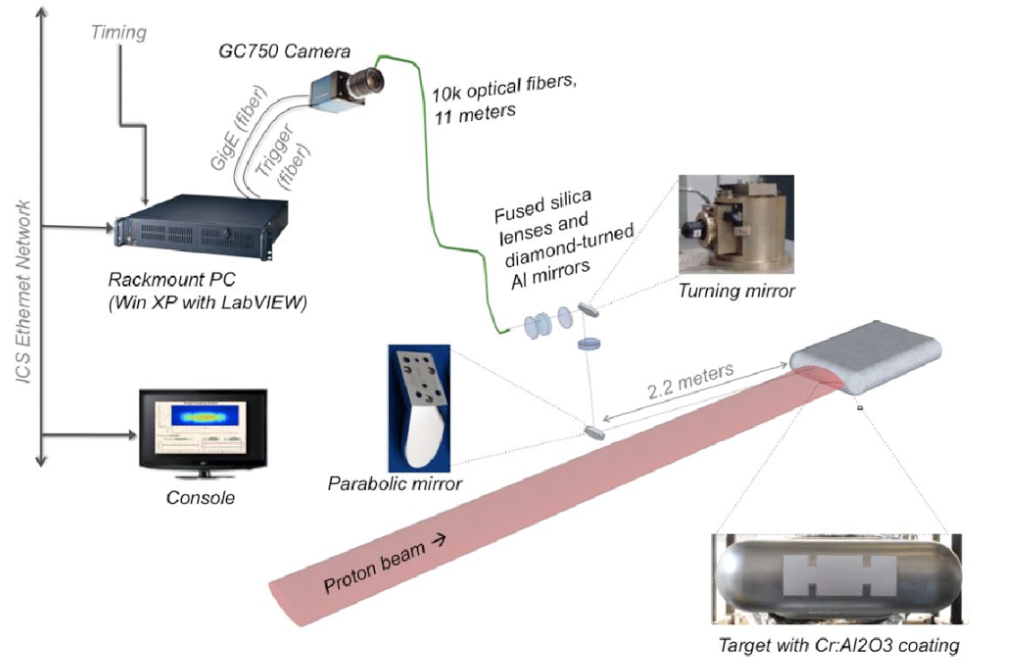
\includegraphics[width=\textwidth]{Images/chapter4/tis1.png}
        \caption{}
        \label{fig:tis_a}
    \end{subfigure}
    \vfill
    \vspace*{2.0cm}
    \vfill
    \begin{subfigure}{0.5\textwidth}
        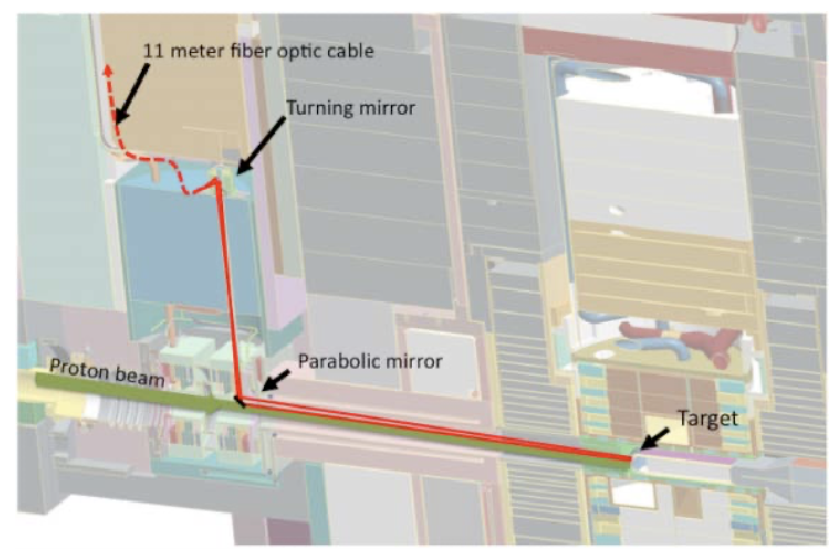
\includegraphics[width=\textwidth]{Images/chapter4/tis2.png}
        \caption{}
        \label{fig:tis_b}
    \end{subfigure}
    \caption{(a) Configuration of the SNS target imaging system. (b) View of the optical path with shielding. (From \cite{Blokland2010}.)}
    \label{fig:tis}
\end{figure}
%

The optics in the RTBT region can be modified, but there are constraints. The $\beta$ functions should be kept below $\approx$ 35 m/rad in the wire-scanner region and below $\approx$ 100 m/rad closer to the target to avoid excess beam loss. At the target, it is best to keep the $\beta$ functions near their default values of $\beta_x \approx$ 60 m/rad and $\beta_y \approx$ 6 m/rad to satisfy peak density requirements on the target. In addition to these constraints, quadrupoles in the wire-scanner region share power supplies. There is a horizontal group \{QH18, QH20, QH22, QH24\} and a vertical group \{QV19, QV21, QV23, QV25\}. The last five magnets — QH26, QV27, QH28, QV29, and QH30 — are individually controlled.


\section{Phase space reconstruction from 1D projections}

\subsection{Method description}

The covariance matrix $\bm{\Sigma}$ can be reconstructed from 1D projections \cite{book:Minty2003, Woodley2000, Prat2014}. We seek to reconstruct $\bm{\Sigma}$ at position $a$ by measuring $\langle{xx}\rangle$, $\langle{yy}\rangle$ and $\langle{xy}\rangle$ at postion $b$, downstream of $A$. Assuming linear transport, the two covariance matrices are related by
%
\begin{equation}
    \bm{\Sigma}_b = \mathbf{M} \bm{\Sigma}_a \mathbf{M}^T,
\end{equation}
%
where $\mathbf{M}$ is the linear transfer matrix from $a$ to $b$. We repeat the measurement at least four times with different transfer matrices — either by changing the measurement location or by changing machine optics — and write
%
\begin{equation}
    \begin{bmatrix}
        {\langle{xx}\rangle}^{(1)} \\
        {\langle{xy}\rangle}^{(1)} \\
        {\langle{yy}\rangle}^{(1)} \\
        {\langle{xx}\rangle}^{(2)} \\
        {\langle{xy}\rangle}^{(2)} \\
        {\langle{yy}\rangle}^{(2)} \\
        {\langle{xx}\rangle}^{(3)} \\
        {\langle{xy}\rangle}^{(3)} \\
        {\langle{yy}\rangle}^{(3)} \\
        \vdots
    \end{bmatrix}_b
    = \mathbf{A}
    \begin{bmatrix}
        \langle{xx}\rangle \\
        \langle{xx'}\rangle \\
        \langle{xy}\rangle \\
        \langle{xy'}\rangle \\
        \langle{x'x'}\rangle \\
        \langle{x'y}\rangle \\
        \langle{x'y'}\rangle \\
        \langle{yy}\rangle \\
        \langle{yy'}\rangle \\
        \langle{y'y'}\rangle \\
    \end{bmatrix}_a
    .
\end{equation}
%
The superscripts represent the measurement index. The coefficient matrix $\mathbf{A}$ for a single measurement is
%
\begin{equation}
    \mathbf{A}^T = 
    \begin{bmatrix}
        M_{11}M_{11} & M_{11}M_{31} & M_{31}M_{31} \\
        2M_{11}M_{12} & M_{12}M_{31} + M_{11}M_{32} & 2M_{31}M_{32} \\
        2M_{11}M_{13} & M_{13}M_{31} + M_{11}M_{33} & 2M_{31}M_{33} \\
        2M_{11}M_{14} & M_{14}M_{31} + M_{11}M_{34} & 2M_{31}M_{34} \\
        M_{12}M_{12} & M_{12}M_{32} & M_{32}M_{32} \\
        2M_{12}M_{13} & M_{13}M_{32} + M_{12}M_{33} & 2M_{32}M_{33} \\
        2M_{12}M_{14} & M_{14}M_{32} + M_{12}M_{34} & 2M_{32}M_{34} \\
        M_{13}M_{13} & M_{13}M_{33} & M_{33}M_{33} \\
        2M_{13}M_{14} & M_{14}M_{33} + M_{13}M_{34} & 2M_{33}M_{34} \\
        M_{14}M_{14} & M_{14}M_{34} & M_{34}M_{34}
    \end{bmatrix}
\end{equation}
%
where $M_{ij}$ is the $i$,$j$ element of the transfer matrix for that measurement. The system is solved using linear least squares (LLSQ). 

The measurement has a geometric interpretation, illustrated in  Fig.~\ref{fig:ws_emittance_measurement} for the 2D case. 
%
\begin{figure}[!p]
    \centering
    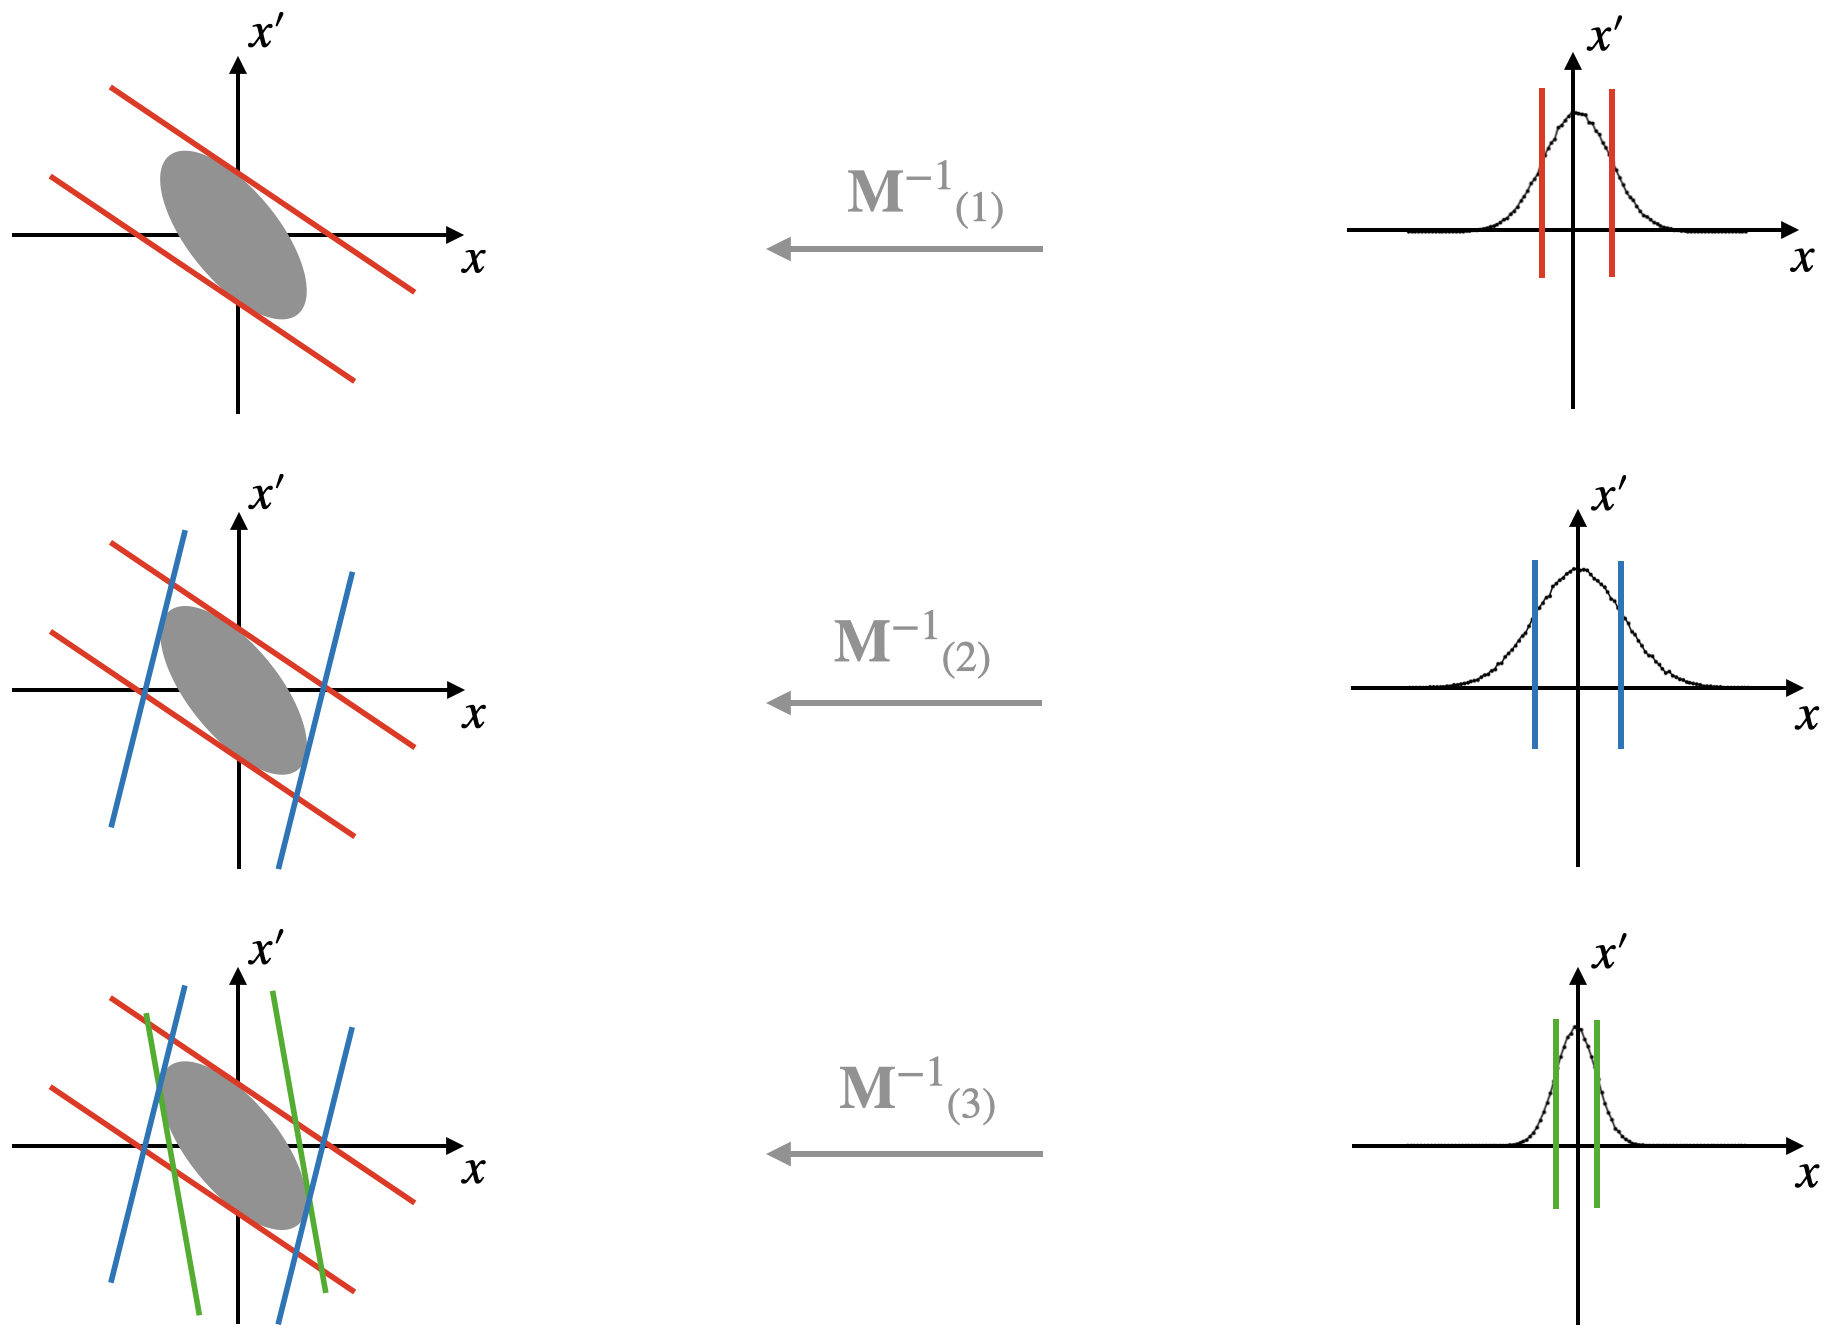
\includegraphics[width=\textwidth]{Images/chapter4/ws_emittance_measurement.png}
    \caption{Illustration of 2D emittance measurement.}
    \label{fig:ws_emittance_measurement}
\end{figure}
%
Each measured beam size defines two lines in the $x$-$x'$ plane at $b$. When the lines are transported back to $a$, their intersection bounds the phase space ellipse. In the general case, each measurement at $b$ defines a 2D surface in 4D phase space (an ellipse in the $x$-$y$ plane with unknown $x'$ and $y'$), and the intersection of these surfaces at $a$ bounds the phase space ellipsoid.


\subsection{Implementation in the SNS}

The four SNS wire-scanners produce four equations, exactly determining the cross-plane moments, so no optics changes are needed in principle; however, additional measurements should reduce the error. In the 2D case, is typically recommended to space $n$ measurements by $\pi / n$ in phase advance \cite{book:Minty2003}. This may be due to the geometric interpretation of Fig.~\ref{fig:ws_emittance_measurement}: in normalized phase space, the rotation angle of the measurement lines is equivalent to the phase advance and the lines are evenly spaced around the phase space ellipse. But in the general case, the angle is given by \cite{Hock2011}
%
\begin{equation}
    \tan\theta = \frac{M_{12}}{M_{11}},
\end{equation}
%
so the spacing will not be uniform. This issue should therefore be investigated numerically in each lattice. The four wire-scanners in the RTBT are already somewhat evenly spaced in phase advance, and it was determined that a 30$\degree$ window around each wire-scanner would provide sufficient coverage. 

Another option, recognized late in this research project, is to compute the RMS moments from the images of the distribution on the target. These images can be collected rapidly, and the $x$-$y$ correlation is computed directly instead of indirectly using a diagonal wire. The use of target images will be explored in the next chapter; the rest of this section focuses only on the wire-scanner measurement.

Due to the shared power supplies of the quadrupoles in the wire-scanner region, there is limited control of the phase advances between the wire-scanners. We instead vary the horizontal and vertical phase advances from QH18 (the first varied quadrupole) to WS24 (the last wire-scanner). This changes the phase advances at WS20, WS21, and WS23 by approximately the same amount. 

To set the phase advances at WS24 while constraining the beam size in the wire-scanner region, the two power supplies (eight quadrupoles) upstream of WS24 were varied using an optimizer that minimizes the following cost function:
%
\begin{equation}
    C(\mathbf{g}) = \left\Vert{\tilde{\bm{\mu}} - \bm{\mu} }\right\Vert^2
    + 
    \epsilon
    \left\Vert
    \Theta\left(
        \tilde{\bm{\beta}}_{max} - \bm{\beta}_{max}
    \right)
    \right\Vert^2
    .
\end{equation}
%
The quadrupole field strengths are contained in the vector $\mathbf{g}$. The calculated and desired phase advances at WS24 are $\bm{\mu} = (\mu_x, \mu_y)$, and $\tilde{\bm{\mu}} = (\tilde{\mu}_x, \tilde{\mu}_y)$, respectively. The maximum calculated and allowed $\beta$ functions in the wire-scanner region are $\bm{\beta} = (\beta_{x_{max}}, \beta_{y_{max}})$ and $\tilde{\bm{\beta}}_{max} = (\tilde{\beta}_{x_{max}}, \tilde{\beta}_{y_{max}})$, respectively. $\Theta$ is the Heaviside step function. Finally, $\epsilon$ is a constant. It is hoped that the beam is matched to the lattice optics so that the calculated phase advances are close to the true phase advances.

A GUI application was developed in the OpenXAL framework for use in the SNS control room. In the first pane of the application, the user can set the phase advances at WS24 and view the model optics and phase advances throughout the RTBT. In the second pane, the user can load wire-scanner output files and choose the reconstruction location. These files are output from a separate application and contain the wire-scanner profiles, RMS parameters, and Gaussian fit parameters. They also contain a number that defines the machine state — magnet strengths, etc. — at the time of the measurement. The application reads this number, synchronizes the model with the machine state, and computes the transfer matrices from the wire-scanners to the reconstruction location. The RMS moments and transfer matrices are then used to reconstruct the covariance matrix. The resulting beam parameters are printed and compared to the model lattice parameters. The 2D projections of the covariance ellipsoid are plotted along with the measurement lines, with the option to view in normalized coordinates. 



\subsection{Measurement of a production beam}

The multi-optics method was tested on a fully accumulated production beam. The phase advances at WS24 were varied in a 30$\degree$ range over ten steps — the first half of the scan held the vertical phase fixed while varying the horizontal phase, and the second half of the scan held the horizontal phase fixed while varying the vertical phase. The results of the reconstruction are shown in Fig.~\ref{fig:prod_meas} for a location just before QH18.
%
\begin{figure}[!p]
    \centering
    \begin{subfigure}{0.8\textwidth}
        \centering
        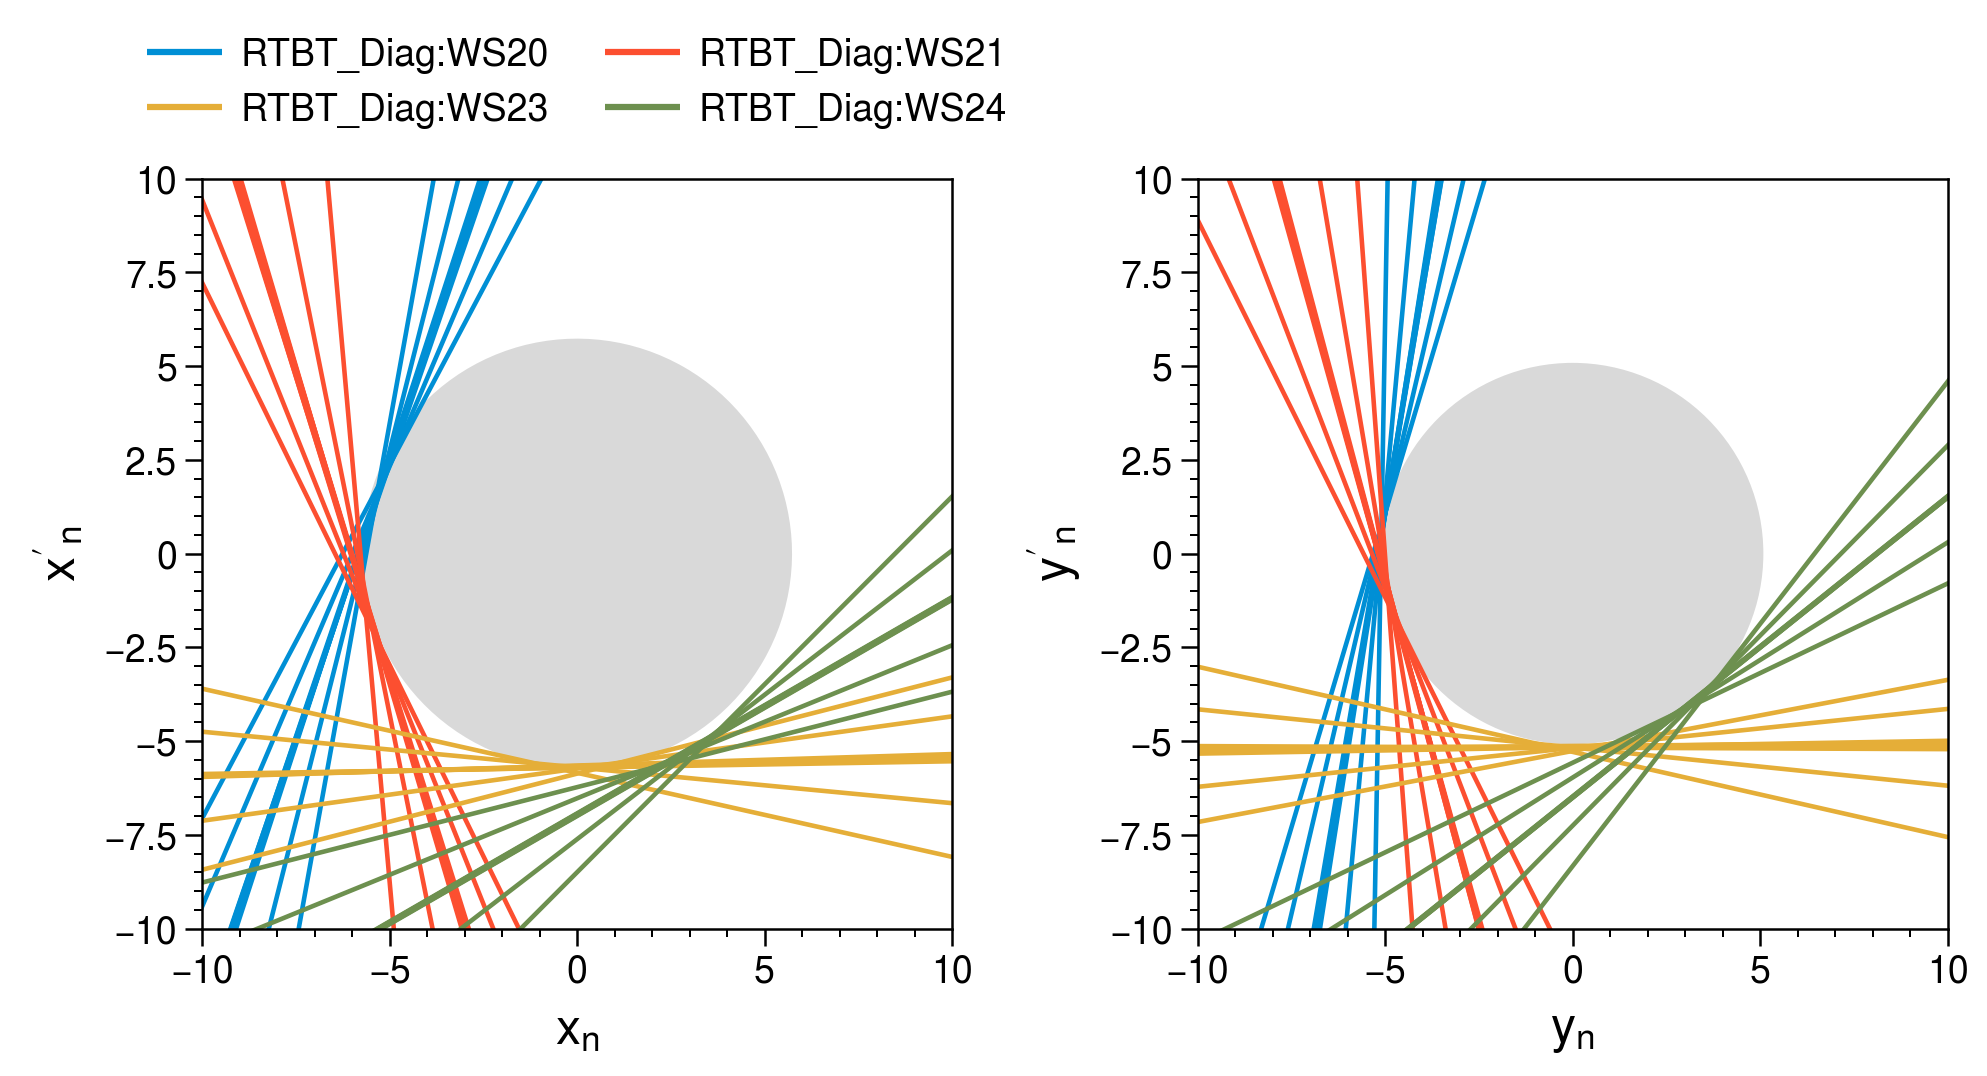
\includegraphics[width=\textwidth]{Images/chapter4/prod_meas_lines.png}  
    \end{subfigure}
    \par\medskip
    \begin{subfigure}{0.6\textwidth}
        \centering
        \begin{tabular}{lcc}
            \small\textbf{Parameter} & \small\textbf{Measurement} & \small\textbf{Model} \\
            \midrule
            \small$\beta_x$ [m/rad] & \small22.06 $\pm$ 0.29 & \small22.00 \\
            \small$\beta_y$ [m/rad] & \small4.01 $\pm$ 0.02 & \small3.81 \\
            \small$\alpha_x$ [rad] & \small2.33 $\pm$ 0.04 & \small2.37 \\
            \small$\alpha_y$ [rad] & \small-0.49 $\pm$ 0.01 & \small-0.60 \\
            \small$\varepsilon_1$ [mm~mrad] & \small33.02 $\pm$ \small0.05 & - \\
            \small$\varepsilon_2$ [mm~mrad] & \small25.67 $\pm$ \small1.03 & - \\
            \small$\varepsilon_x$ [mm~mrad] & \small32.85 $\pm$ \small0.05 & - \\
            \small$\varepsilon_y$ [mm~mrad] & \small25.87 $\pm$ \small0.12 & - \\
          \end{tabular}
    \end{subfigure}
    \par\medskip
    \caption{Reconstructed beam parameters and graphical output from a multi-optics emittance measurement of a production beam.}
    \label{fig:prod_meas}
\end{figure}
%
The best-fit ellipses in the $x$-$x'$ and $y$-$y'$ planes are normalized by the reconstructed Twiss parameters. The uncertainties in the beam parameters were calculated by propagating the standard deviations of the ten reconstructed moments obtained from the LLSQ estimator. The reconstructed Twiss parameters are close to the model parameters computed from the linear transfer matrices of the ring and RTBT, showing that the beam is matched. The intrinsic emittances are almost equal to the apparent emittances, showing that there is very little cross-plane correlation. This is expected for a production beam.

Decreasing the number of measurements used in the reconstruction had no substantial effect on the answer as long as at least two measurements (eight profiles) were used; however, the fit usually failed when only one measurement (four profiles) was used. Here, ``failed fit" means that the reconstructed covariance matrix is unphysical, producing imaginary intrinsic emittances. 



\subsection{Sensitivity to measurement errors}

A nonlinear solver can be used to ensure that the reconstructed covariance matrix is physical; however, the answer was found to depend strongly on the initial guess provided to the solver. To investigate the failure of the fixed-optics method, the reconstructed covariance matrix (using the full data set) was tracked to the wire-scanners using the known transfer matrices. Random Gaussian noise was added to the moments at these locations, and the noisy moments were used to perform the reconstruction. This was repeated for several trials. It was found that the reconstruction was extremely sensitive to changes in the beam moments, as shown in Fig.~\ref{fig:prod_sensitivity}.
%
\begin{figure}[!p]
    \centering
    \begin{subfigure}{1.0\textwidth}
        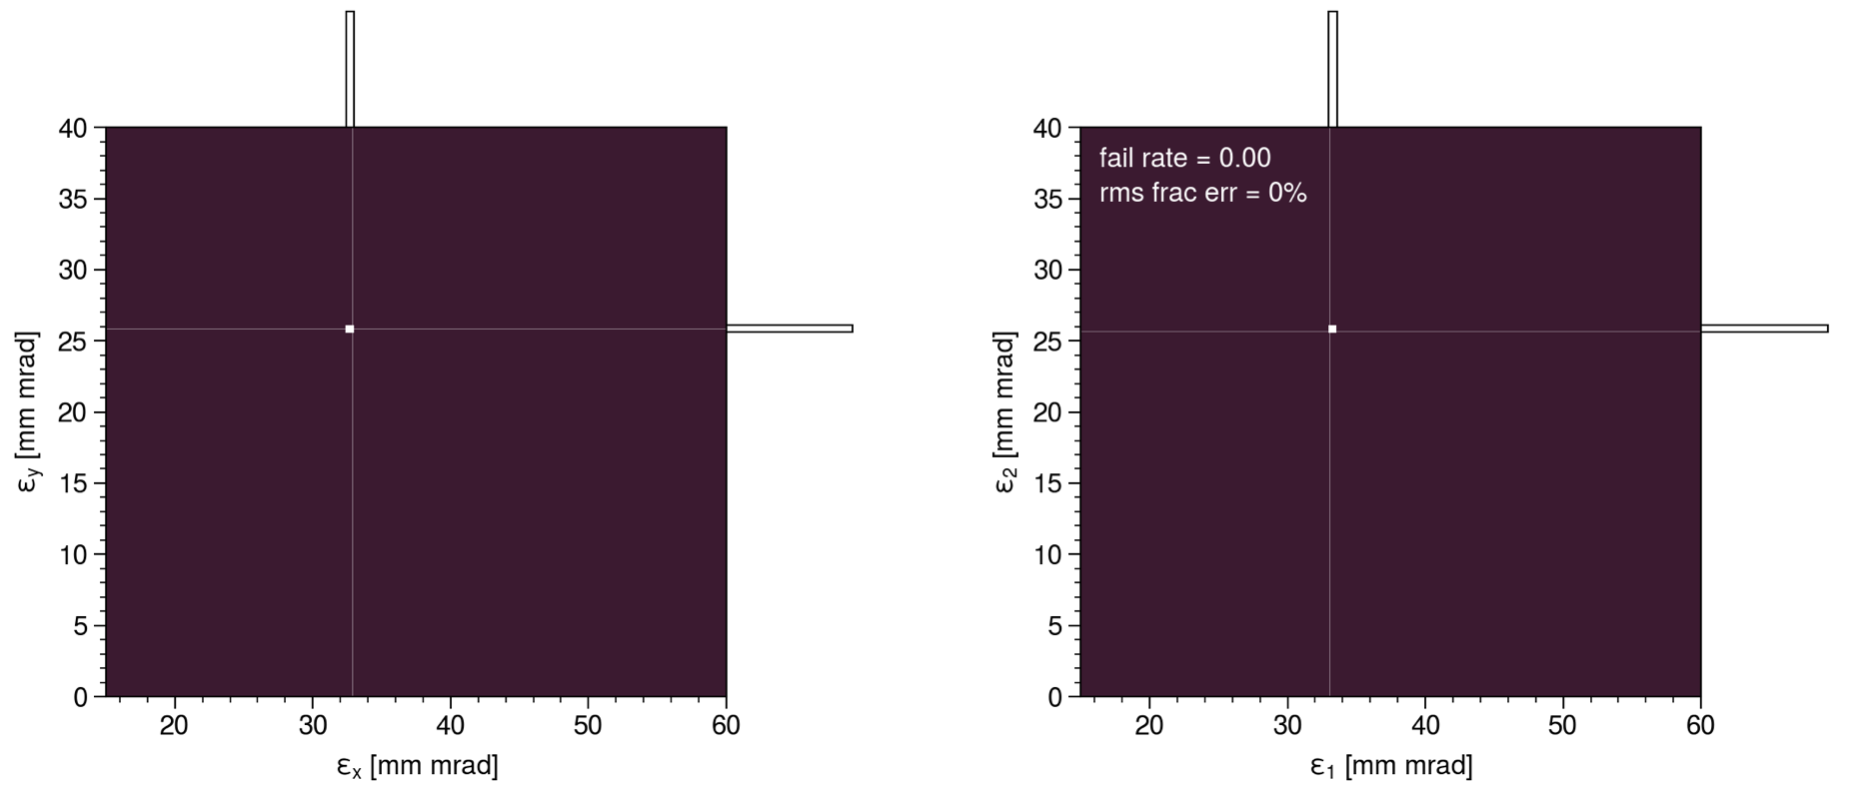
\includegraphics[width=\textwidth]{Images/chapter4/prod_sensitivity1.png}
    \end{subfigure}
    \vfill
    \vspace*{0.5cm}
    \vfill
    \begin{subfigure}{1.0\textwidth}
        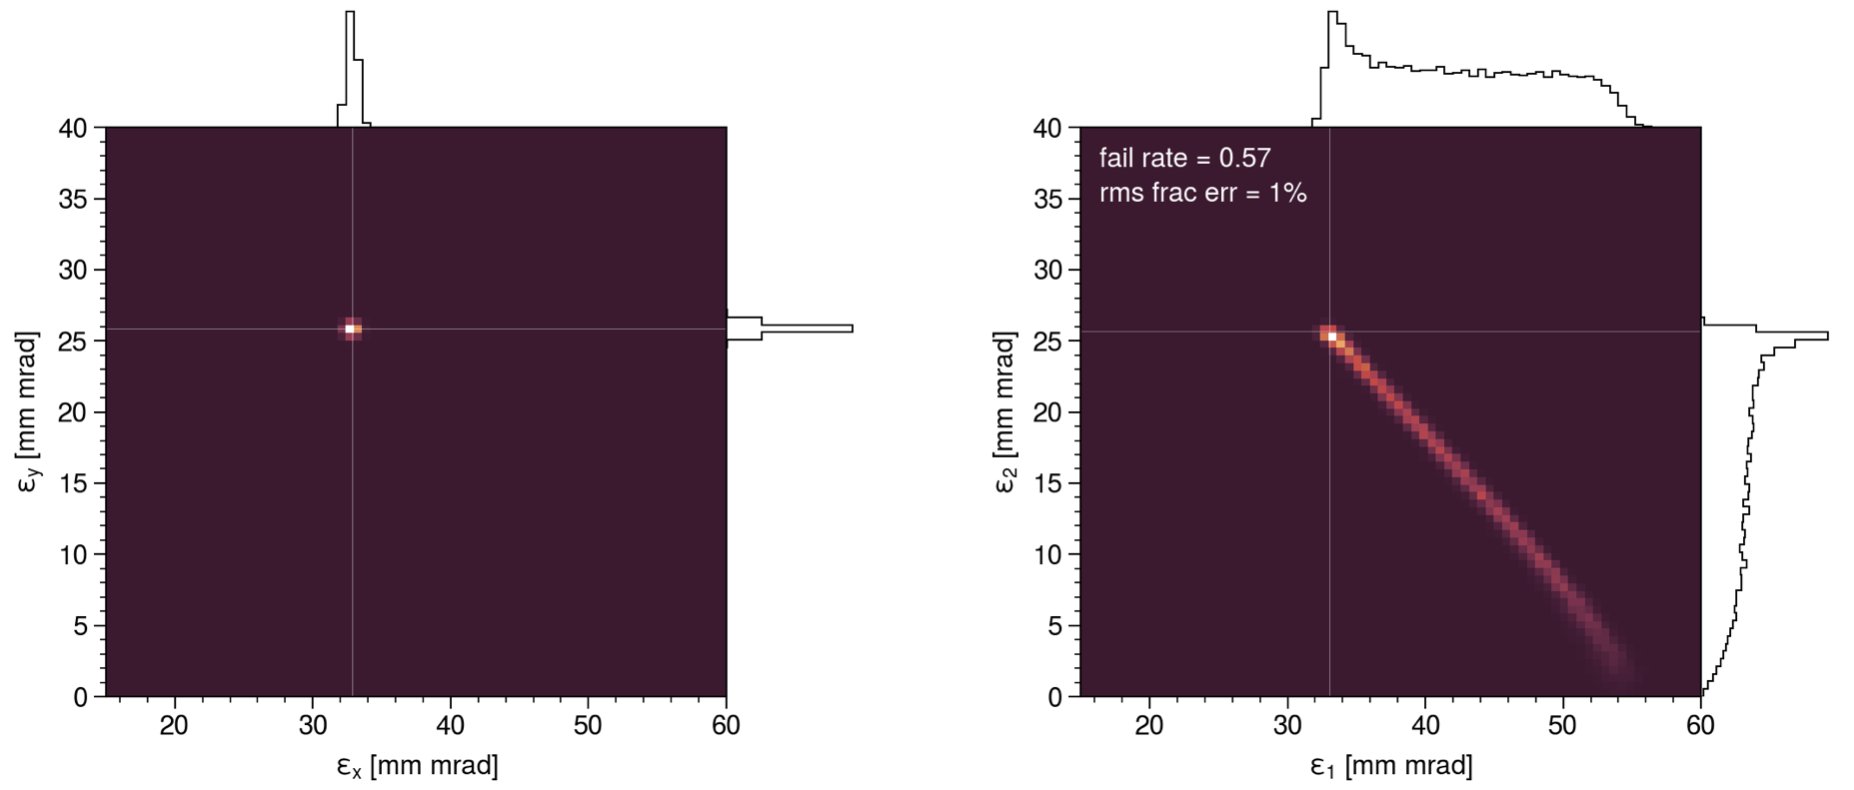
\includegraphics[width=\textwidth]{Images/chapter4/prod_sensitivity2.png}
    \end{subfigure}
    \vfill
    \vspace*{0.5cm}
    \vfill
    \begin{subfigure}{1.0\textwidth}
        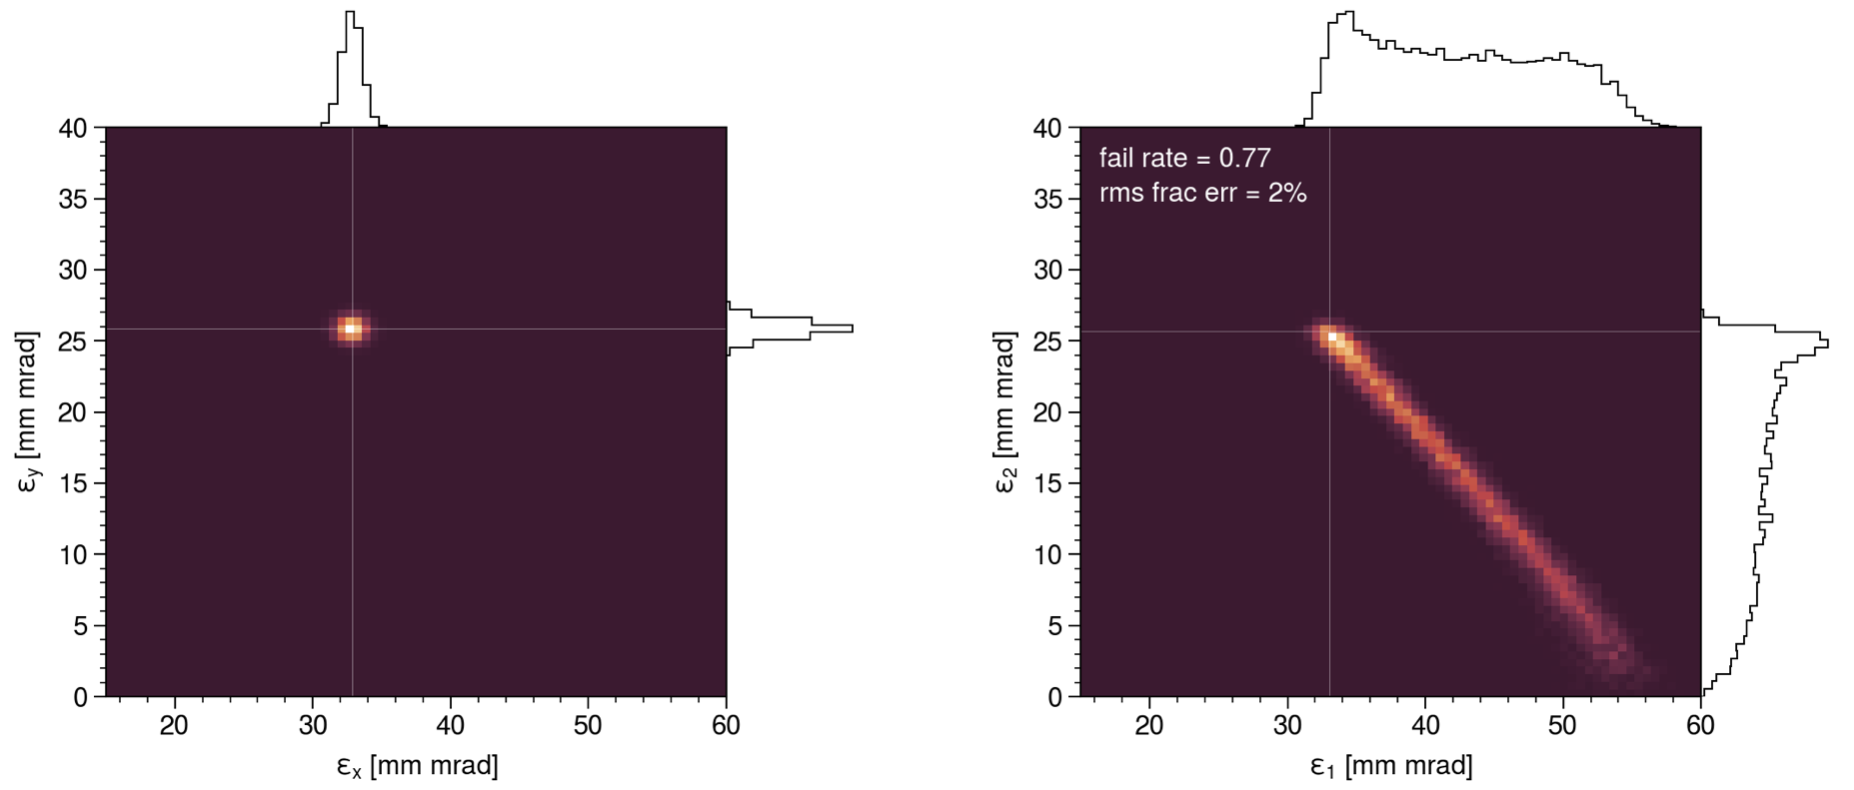
\includegraphics[width=\textwidth]{Images/chapter4/prod_sensitivity3.png}
    \end{subfigure}
    \caption{Monte Carlo trials of a fixed-optics emittance measurement in the RTBT. Left: apparent emittances.}
    \label{fig:prod_sensitivity}
\end{figure}
%
As soon as any noise is included, the fail rate jumps to a large value; additionally, the intrinsic emittances reconstructed in the successful fits have a large, asymmetric spread around the correct values. On the other hand, the apparent emittances are localized around the correct values. (The transfer matrices are uncoupled, so the $x$-$x'$ and $y$-$y'$ reconstructions are performed independently. The problem is with the cross-plane moments.)

Sensitivity of 4D emittance measurements using fixed-optics was observed in \cite{Woodley2000}, including the asymmetric distribution of errors in Fig.~\ref{fig:prod_meas}. The problem was studied more recently in \cite{Agapov2007} and \cite{Faus-Golfe2016}. The conclusion from these studies is that the linear system for the cross-plane moments is ill-conditioned. The sensitivity of a linear system $\mathbf{A} \mathbf{x} = \mathbf{b}$ to errors in $\mathbf{b}$ is determined by the condition number of $\mathbf{A}$, which is the product of matrix norms $\Vert \mathbf{A} \Vert \Vert \mathbf{A}^{-1} \Vert$. As an example, consider four wire-scanners that are evenly spaced in phase advance and connected by rotation matrices. Fig.~\ref{fig:fodo_condition_number} plots the condition number of the coefficient matrix as a function of the spacing between the wire-scanners.
%
\begin{figure}[!p]
    \centering
    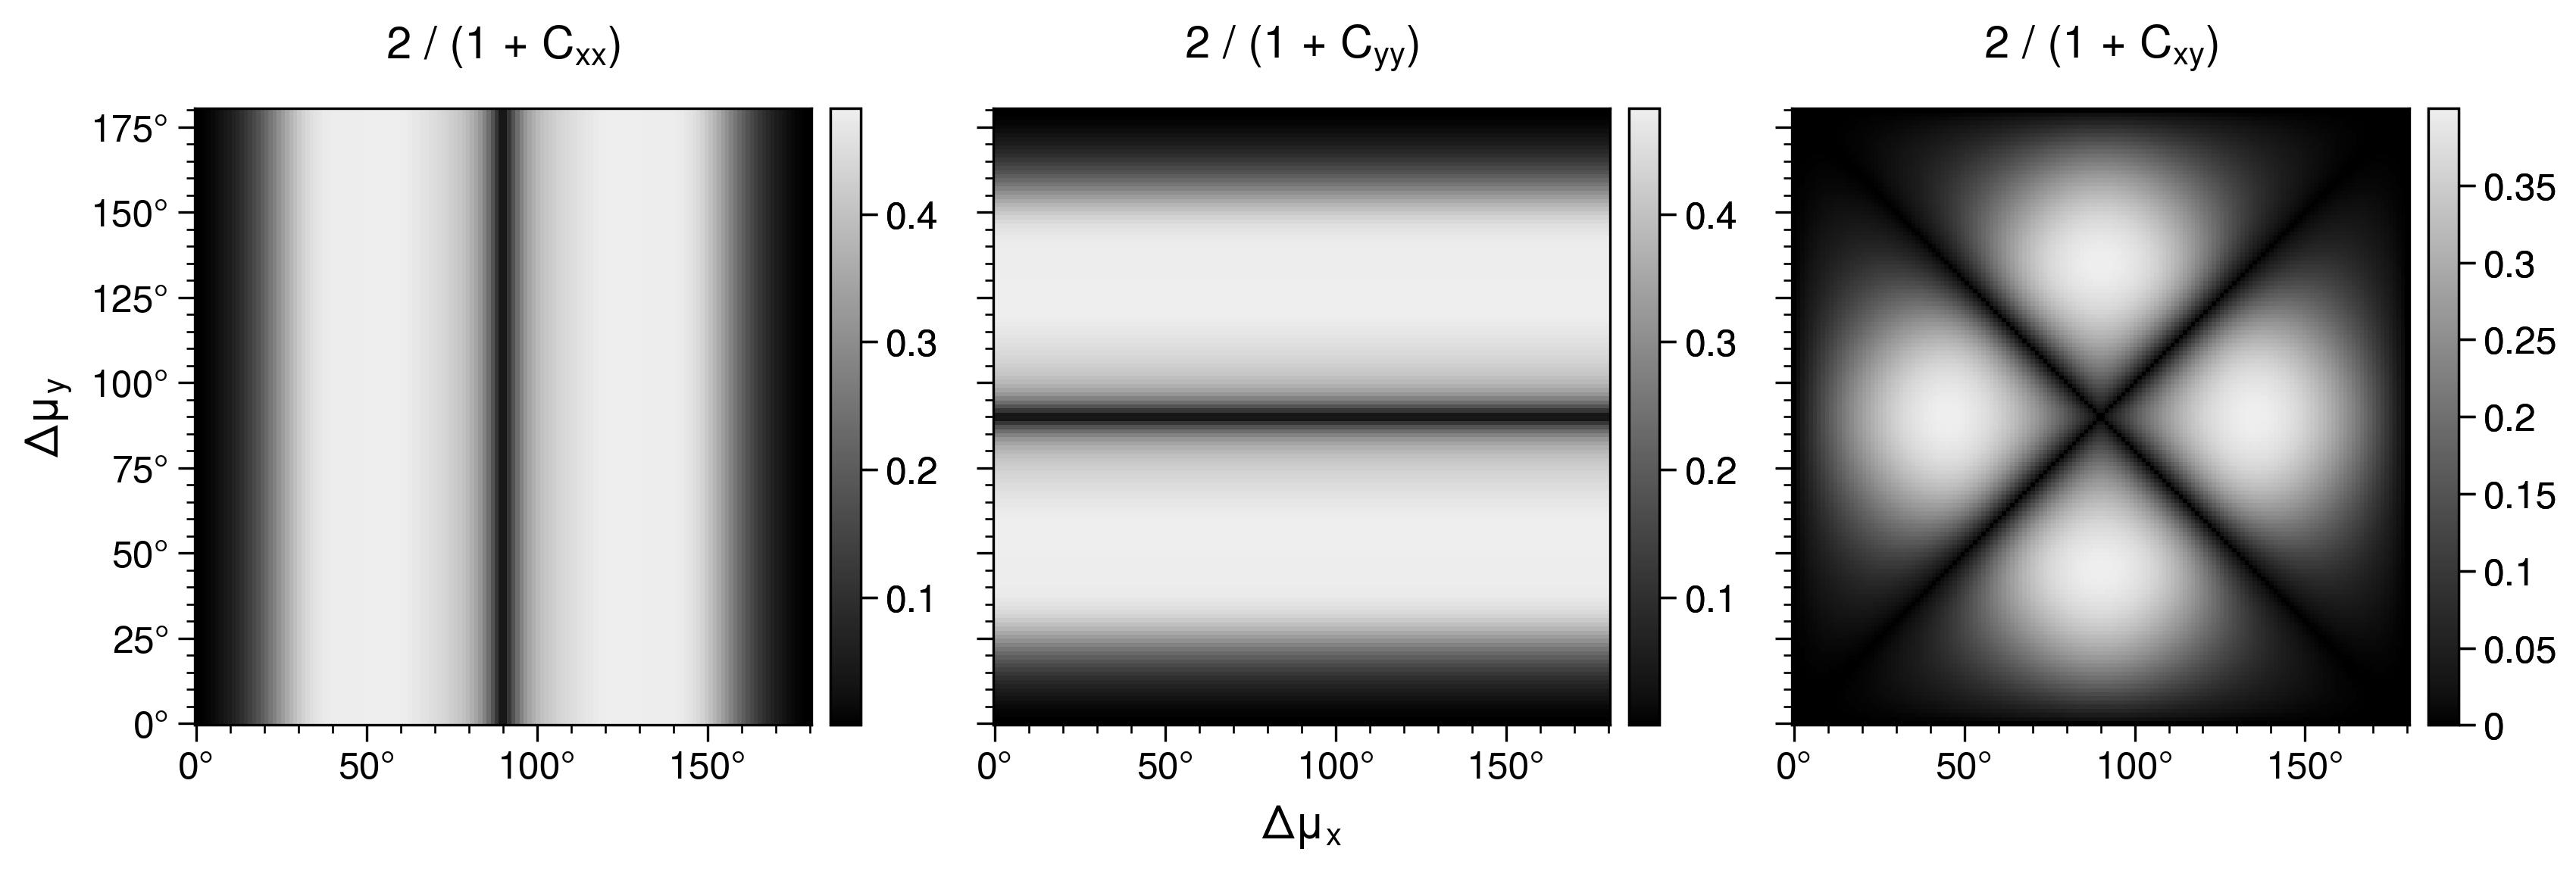
\includegraphics[width=0.7\textwidth]{Images/chapter4/fodo_condition_number.png}
    \caption{Condition number $C$ of the coefficient matrix for four wire-scanners that are evenly spaced in phase advance and connected by rotation matrices.}
    \label{fig:fodo_condition_number}
\end{figure}
%
The condition number is large when the spacing is 90\degree, in which case the two measurements provide degenerate information in $x$-$x'$ or $y$-$y'$. The sum and difference lines correspond to the cross-plane moments. The chart will be more complicated for different optics or additional wire-scanners.

Fig.~\ref{fig:rtbt_condition_number} shows a similar calculation in the RTBT. 
%
\begin{figure}[!p]
    \centering
    \begin{subfigure}{0.75\textwidth}
        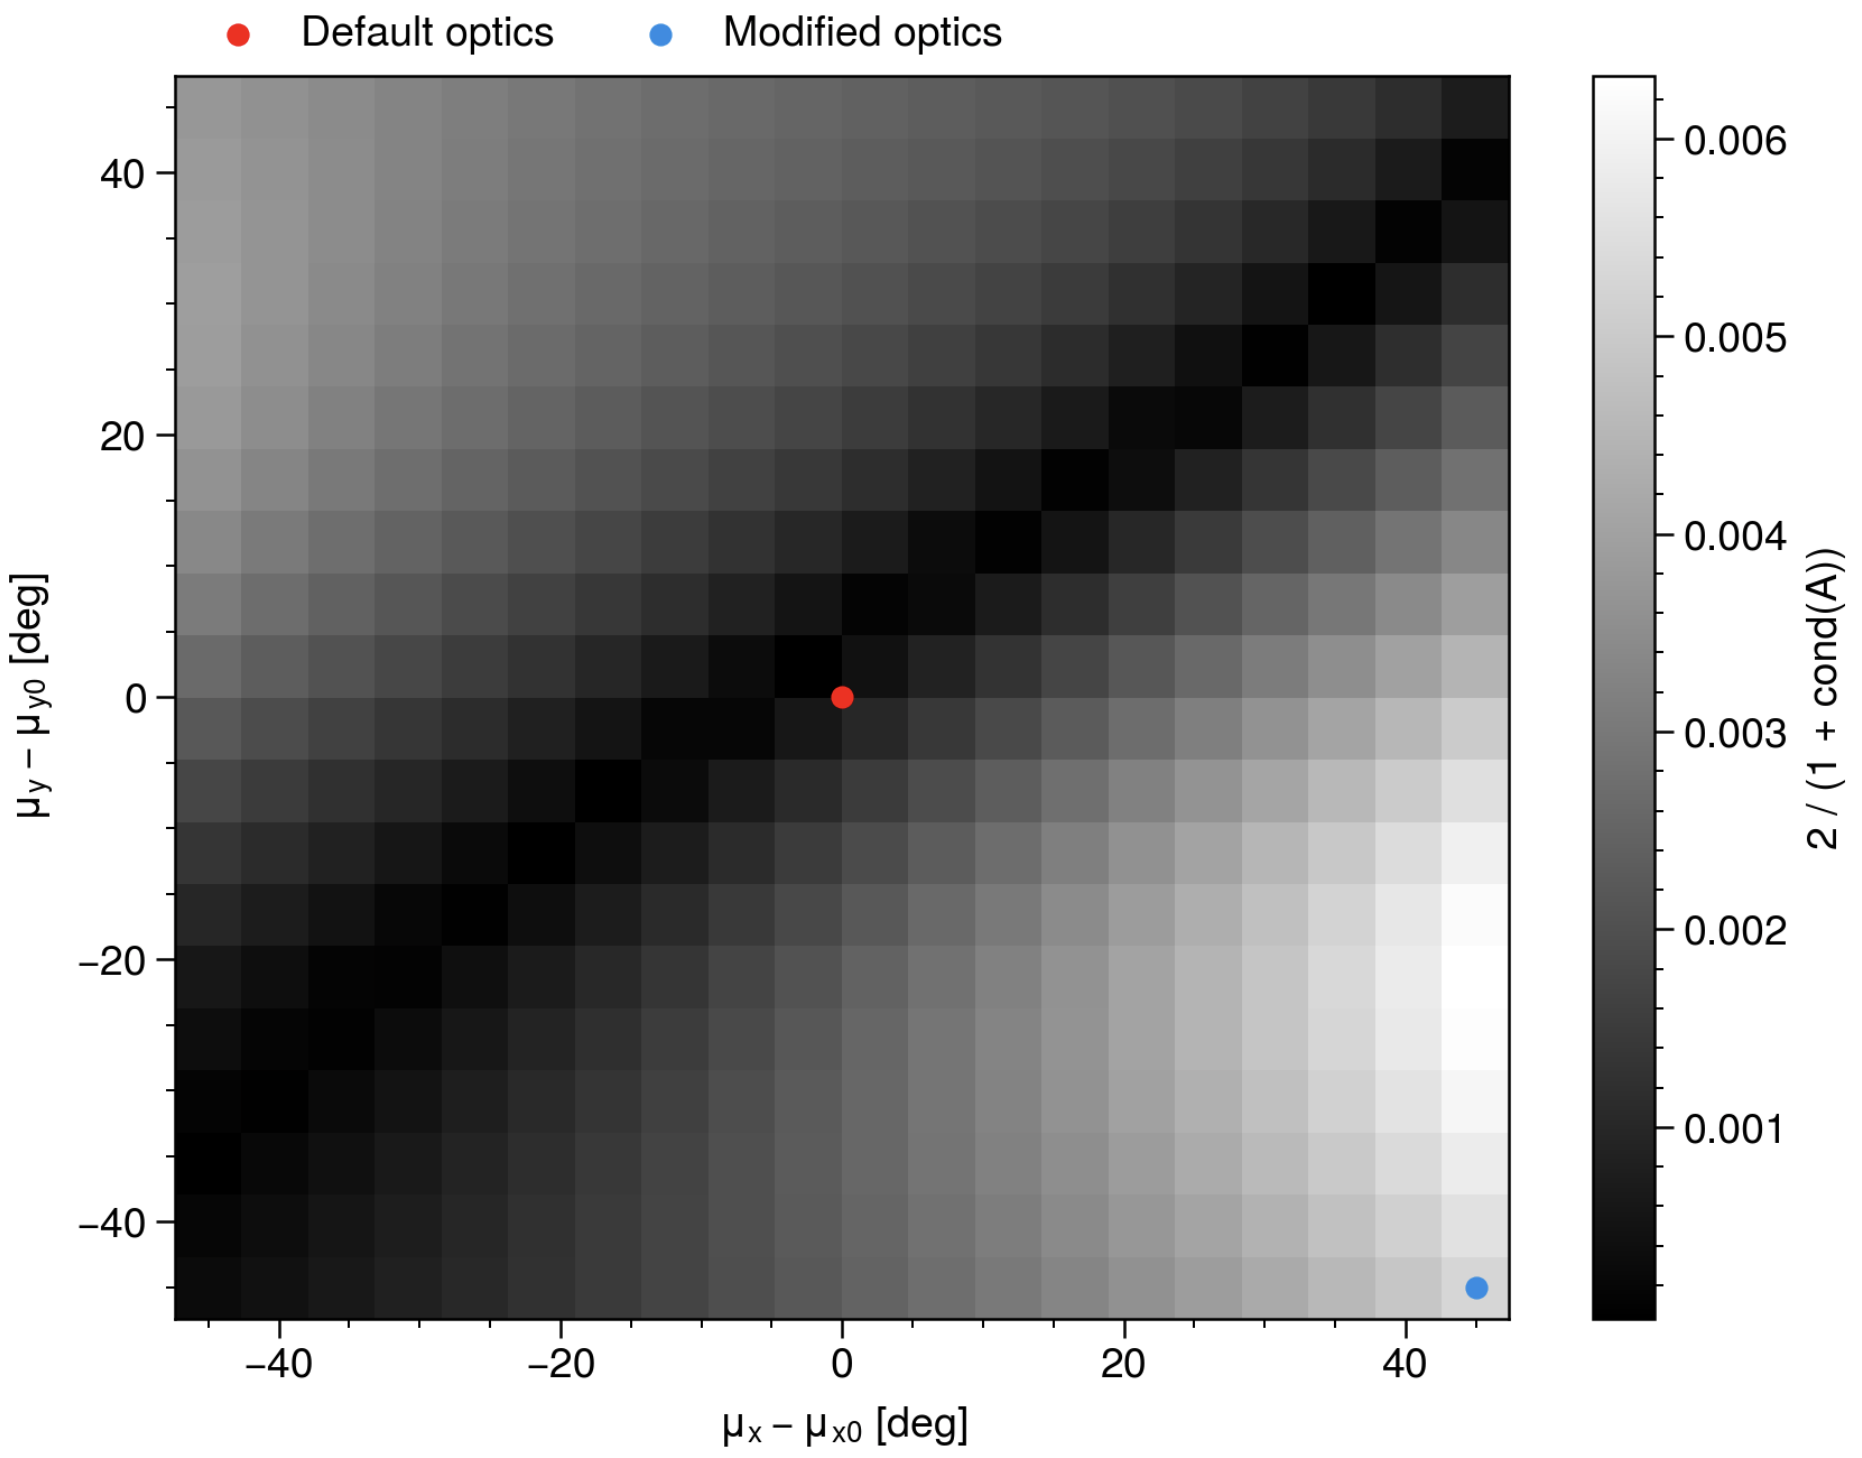
\includegraphics[width=1.0\textwidth]{Images/chapter4/rtbt_condition_number.png}
    \end{subfigure}
    \vfill
    \vspace*{0.8cm}
    \begin{subfigure}{0.75\textwidth}
        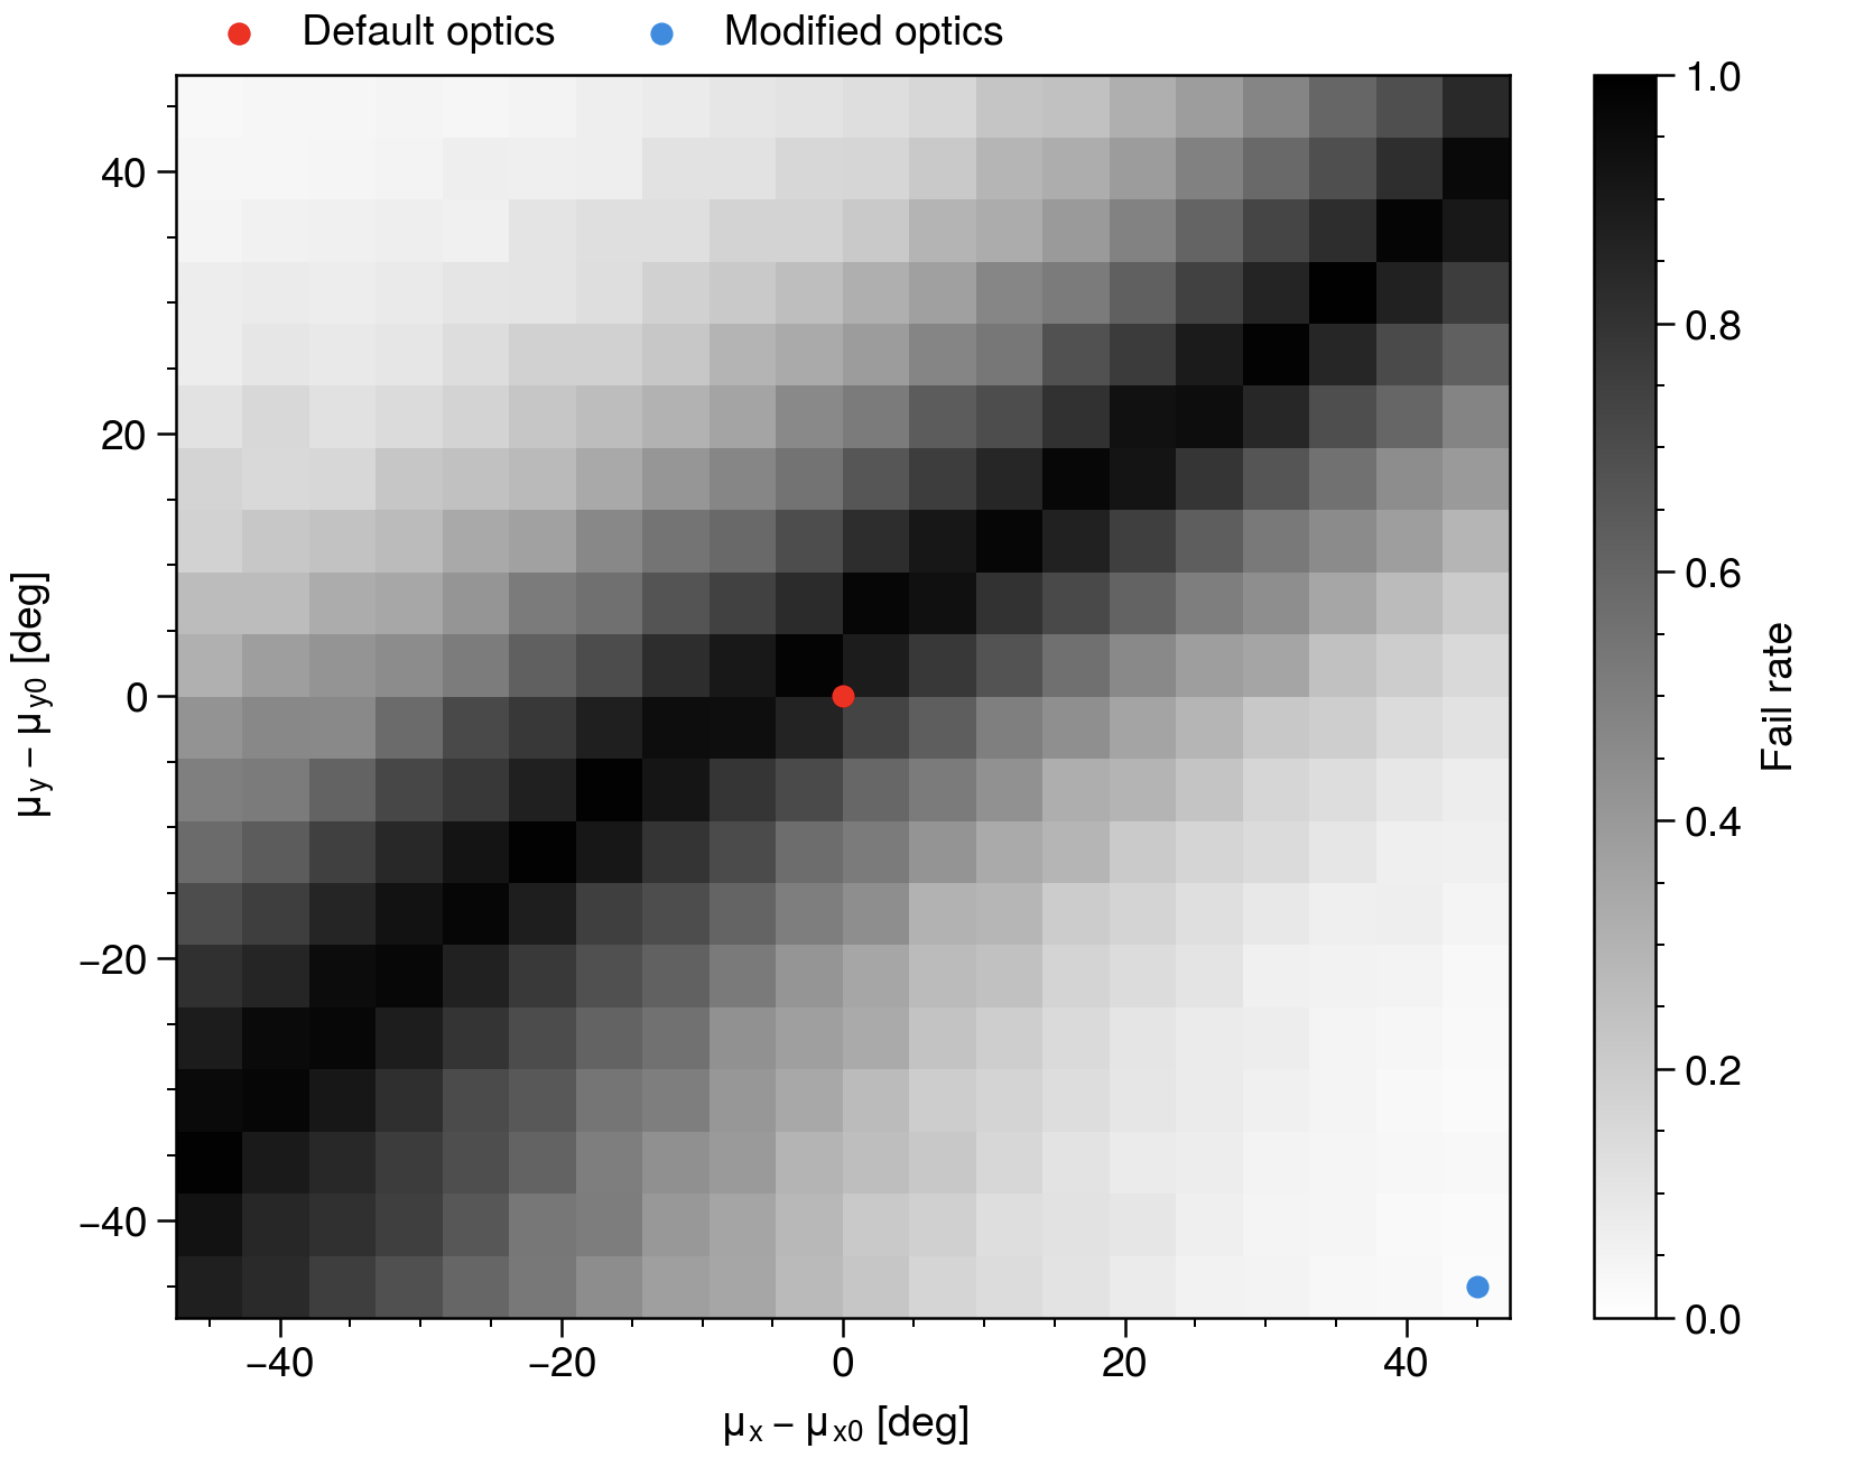
\includegraphics[width=1.0\textwidth]{Images/chapter4/rtbt_fail_rate.png}
    \end{subfigure}
    \caption{4D emittance reconstruction errors as a function of the phase advances at WS24. Top: condition number of the linear system. Bottom: simulated reconstruction fail rate with 3\% beam size error.}
    \label{fig:rtbt_condition_number}
\end{figure}
%
The phase advances at WS24 are scanned around their default values. The default optics are ill-suited for the measurement. A new operating point was chosen at the blue dot in the figure. This corrected the issue of failed fits in the following experiments. 
% [Unfortunately, the sensitivity of the successful fits to errors — i.e., the variance of the reconstructed emittances — was not examined in detail. We will return to this point in Chapter \ref{chap-5}].

Finally, we mention that there is information to be gained from 1D projections of the distribution in addition to the RMS reconstruction. The distributions can be compared to the ideal ``half-circle" projections of a uniform density ellipse. The horizontal and vertical projections can be used to reconstruct the $x$-$x'$ or $y$-$y'$ distribution using the tomographic methods described in the next section. It may be possible to include cross-plane information in the reconstruction using the diagonal projections. There is a particular method that can, in principle, reconstruct the $x$-$x'$-$y$-$y'$ distribution from only 1D projections, although the method is untested. 






\section{Phase space reconstruction from 2D projections}

Tomographic methods are well-established for the reconstruction of 2D phase space distributions from 1D projections in transverse phase space \cite{Hock2014} and longitudinal phase space \cite{Evans2014}. The concept has recently been extended to the reconstruction of the 4D transverse phase space, both in theory and in practice \cite{Hock2013b, Wang2019, Wolski2020}. This section begins with a brief discussion of tomography in two dimensions as applied to particle accelerators, then moves on to describe several 4D reconstruction algorithms. The algorithms are implemented and their accuracy and limitations are discussed. Finally, the use of 4D tomography on images from the SNS target imaging system is discussed.


\subsection{Beam tomography}

Many algorithms exist to reconstruct 2D images from 1D projections, such as filtered back-projection (FBP), algebraic reconstruction (ART) \cite{Slaney1988}, and maximum entropy (MENT) \cite{Minerbo1979}. Projections of an object are normally obtained by illuminating the object at different angles. Although the measured 1D projections of a 2D phase space distribution are always along one direction (the $x$ of $y$ axis), we can take advantage of the known transfer matrix $\mathbf{M}$ between the measurement location $b$ and the reconstruction location $a$. The measured projection at $b$ is
%
\begin{equation}
    p_b(x_b) = \int_{-\infty}^{\infty} f(x_b, x'_b) dx'_b.
\end{equation}
%
The projection at $a$ will be along axis $\tilde{x}_a$, which is rotated at angle $\theta$ above the $x_a$ axis. The angle is computed from the transfer matrix: \cite{Hock2013a}: 
%
\begin{equation}\label{eq:proj_trans_1}
    \tan\theta = \frac{M_{12}}{M_{11}}.
\end{equation}
%
The distance along the projection will be scaled:
%
\begin{equation}\label{eq:proj_trans_2}
    r = \frac{x_b}{\tilde{x}_a} = \sqrt{M_{11}^2 + M_{12}^2}.
\end{equation}
%
The projection must then be scaled to conserve area. The projections at $a$ and $b$ are related by 
%
\begin{equation}\label{eq:proj_trans_3}
    p_a(\tilde{x}_a) = r p_b(r \tilde{x}_a).
\end{equation}
%
Standard tomography algorithms can be applied to the scaled projections.

It is also possible to reconstruct in normalized phase space \cite{Hock2011}. Recall the normalization matrix $\mathbf{V}$ from Eq.~\eqref{eq:CS_parameterization}. In normalized coordinates, the transfer matrix is a rotation matrix by an angle equal to the phase advance. It is straightforward to obtain the projections in the normalized phase space at $a$:
%
\begin{equation}
\begin{aligned}
    \mathbf{x} &\rightarrow \mathbf{M} \mathbf{x}
    = \mathbf{M} \mathbf{V} (\mathbf{V}^{-1} \mathbf{x})
    ,
\end{aligned}
\end{equation}
%
where $\mathbf{V}$ is a function of the Twiss parameters at $a$. The previous equations can be applied to the new matrix $\mathbf{M} \mathbf{V}$ to obtain the projections in the normalized phase space at $a$. After the image is reconstructed, the true distribution can be obtained by transforming the grid coordinates using $\mathbf{V}$ and interpolating at the transformed coordinates. Note that any Twiss parameters can be used to form $\mathbf{V}$; if the Twiss parameters are matched to the distribution, the rotation angle of the projection will be the phase advance from $a$ to $b$, and the reconstructed distribution will be circular in the normalized phase space.



\subsection{4D reconstruction as a series of 2D reconstructions}

Recent work by Hock et al. reduces 4D reconstruction to a series of 2D reconstructions when the $x$-$y$ projections are available \cite{Hock2013a}. The method, which we refer to as Hock's method, is as follows. Assume that the horizontal and vertical angles (or phase advances) can be controlled independently. Let the angles in $x$-$x'$ be \{$\theta_{x_1}$, $\dots$, $\theta_{x_k}$, $\dots, \theta_{x_K}$\} and the angles in $y$-$y'$ be \{$\theta_{y_1}$, $\dots$, $\theta_{y_l}$, $\dots$, $\theta_{y_L}$\}. The projections are stored in an array $\mathbf{S}$, where $\mathbf{S}_{i,j,k,l}$ is the intensity at point ($x_i$, $y_j$) on the screen for angles $\theta_x = \theta_{x_k}$, $\theta_y = \theta_{y_l}$. We can immediately reconstruct a 3D projection of the distribution from this data. Consider a single row of the image — the intensity along the row gives a 1D projection onto the $x$ axis for a horizontal slice of the distribution. We have a set of these 1D projections at different $\theta_{x}$ which we can use to reconstruct the $x$-$x'$ distribution at this slice using any 1D $\rightarrow$ 2D reconstruction method. Repeating at each slice gives the array $\mathbf{D}$, where $\mathbf{D}_{j, l, r, s}$ is the density at $x = x_r$, $x' = x'_s$, $y = y_j$, for $\theta_{y} = \theta_{y_l}$. We then analyze the vertical plane. At each bin in the reconstructed $x$-$x'$ grid, we have a set of 1D projections of $y$-$y'$ at each $\theta_{y_l}$, thus, $y$-$y'$ can be reconstructed. This completes the reconstruction: we have an array $\mathbf{Z}$, where $\mathbf{Z}_{r, s, t, u}$ is the density at $x = x_r$, $x' = x_s$, $y = y_t$, $y' = y'_u$.

To test the method, the 600,000-particle distribution from Fig.~\ref{fig:Holmes_corner_compare} was used. In \cite{Hock2013a}, filtered back-projection (FBP) was used in the 2D reconstructions. The disadvantage of FBP is that it requires many projections; simultaneous algebraic reconstruction (SART) is a possible alternative when the number of projections is small. The accuracy of SART will depend on the number of projections and the range of projection angles. Fig.~\ref{fig:tomo_sim_art2D} demonstrates this by reconstructing the $y$-$y'$ distribution from 1D projections as these numbers are varied.
%
\begin{figure}[!p]
    \centering
    \vspace*{3.0cm}
    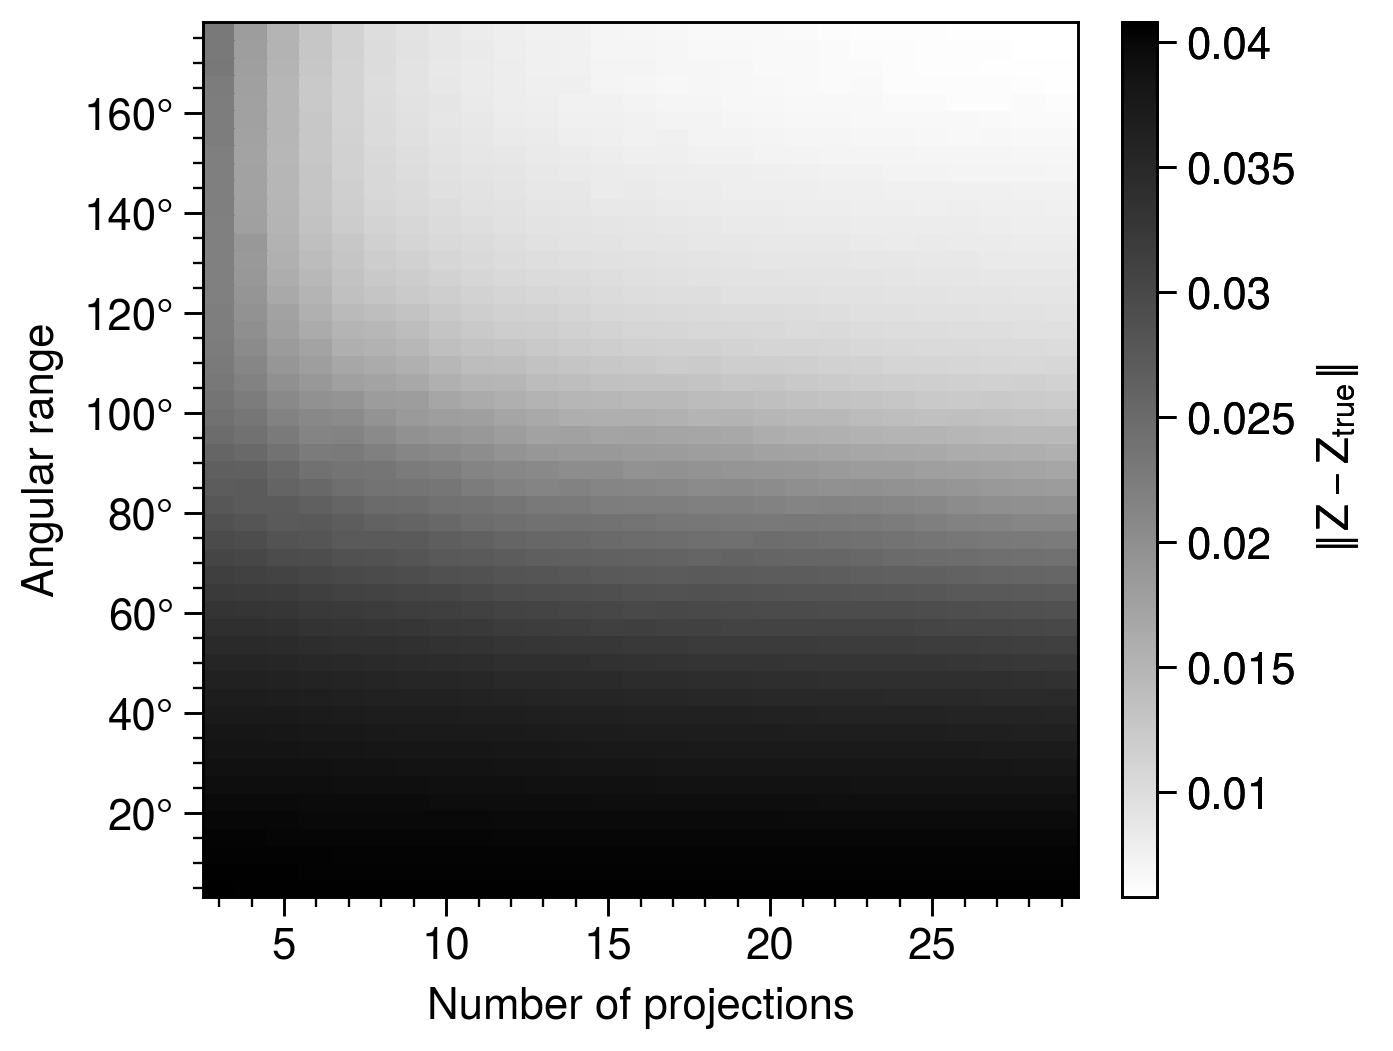
\includegraphics[width=0.6\textwidth]{Images/chapter4/tomo_sim_art2d.png}
    \caption{Test of SART accuracy as a function of number of projections and range of projection angles.}
    \label{fig:tomo_sim_art2D}
    \vspace*{3.0cm}
\end{figure}
%
It appears that if the projection angles are distributed over a significant range, the accuracy does not improve much beyond 10-15 projections. As discussed later, 15 projections is likely near the maximum possible in the SNS. In the following simulated 4D reconstruction, the phase advances in both planes were scanned over $180\degree$ in 12 steps; at each step, the distribution was transported to and then binned on a virtual screen. The reconstruction was performed in normalized phase, and it was assumed that the distribution was matched to the lattice parameters. Fig.~\ref{fig:tomo_sim_target_scan} shows the simulated images in normalized space with a screen resolution of $75 \times 75$.
%
\begin{figure}[!p]
    \centering
    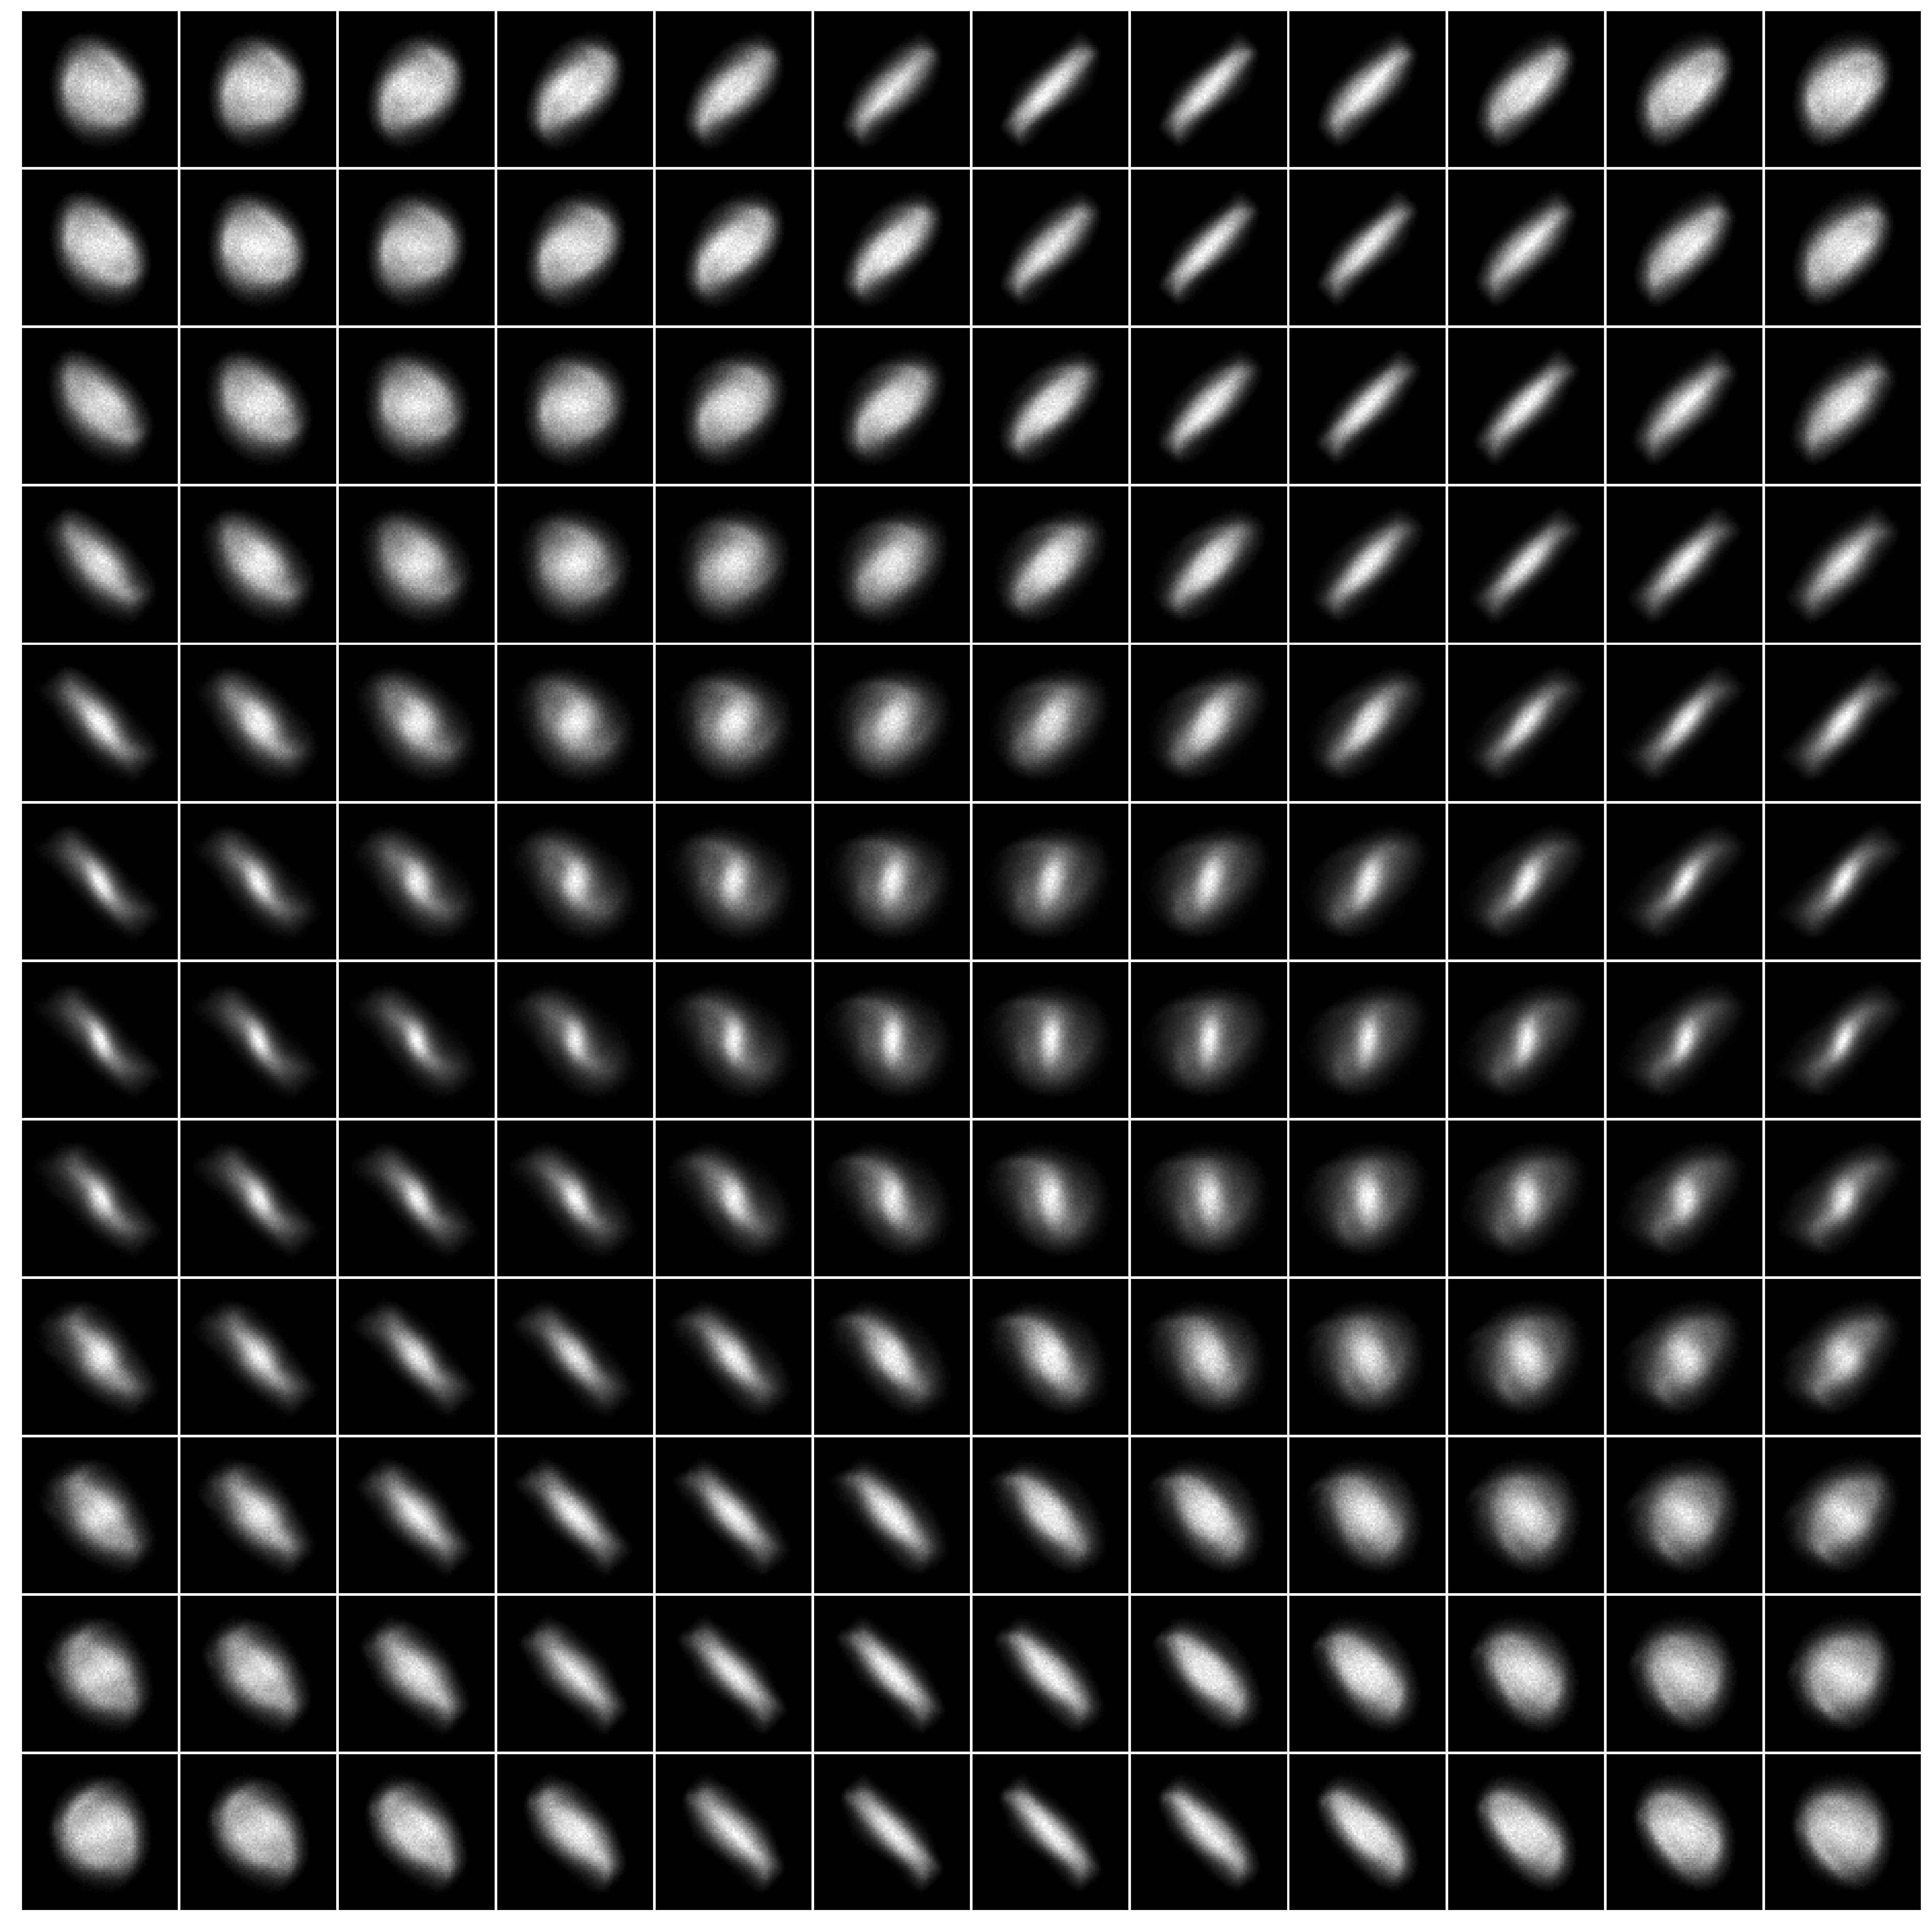
\includegraphics[width=\textwidth]{Images/chapter4/tomo_sim_target_scan_full.png}
    \caption{Simulated $x$-$y$ projections as the horizontal (rows) and vertical (columns) phase advances are varied.}
    \label{fig:tomo_sim_target_scan}
\end{figure}
%
Three SART iterations were used for each 2D reconstruction. The 2D projections of the reconstructed distribution are compared to the original distribution in Fig.~\ref{fig:tomo_sim_rec_hock_proj_2D} in normalized phase space.
%
\begin{figure}[!p]
    \centering
    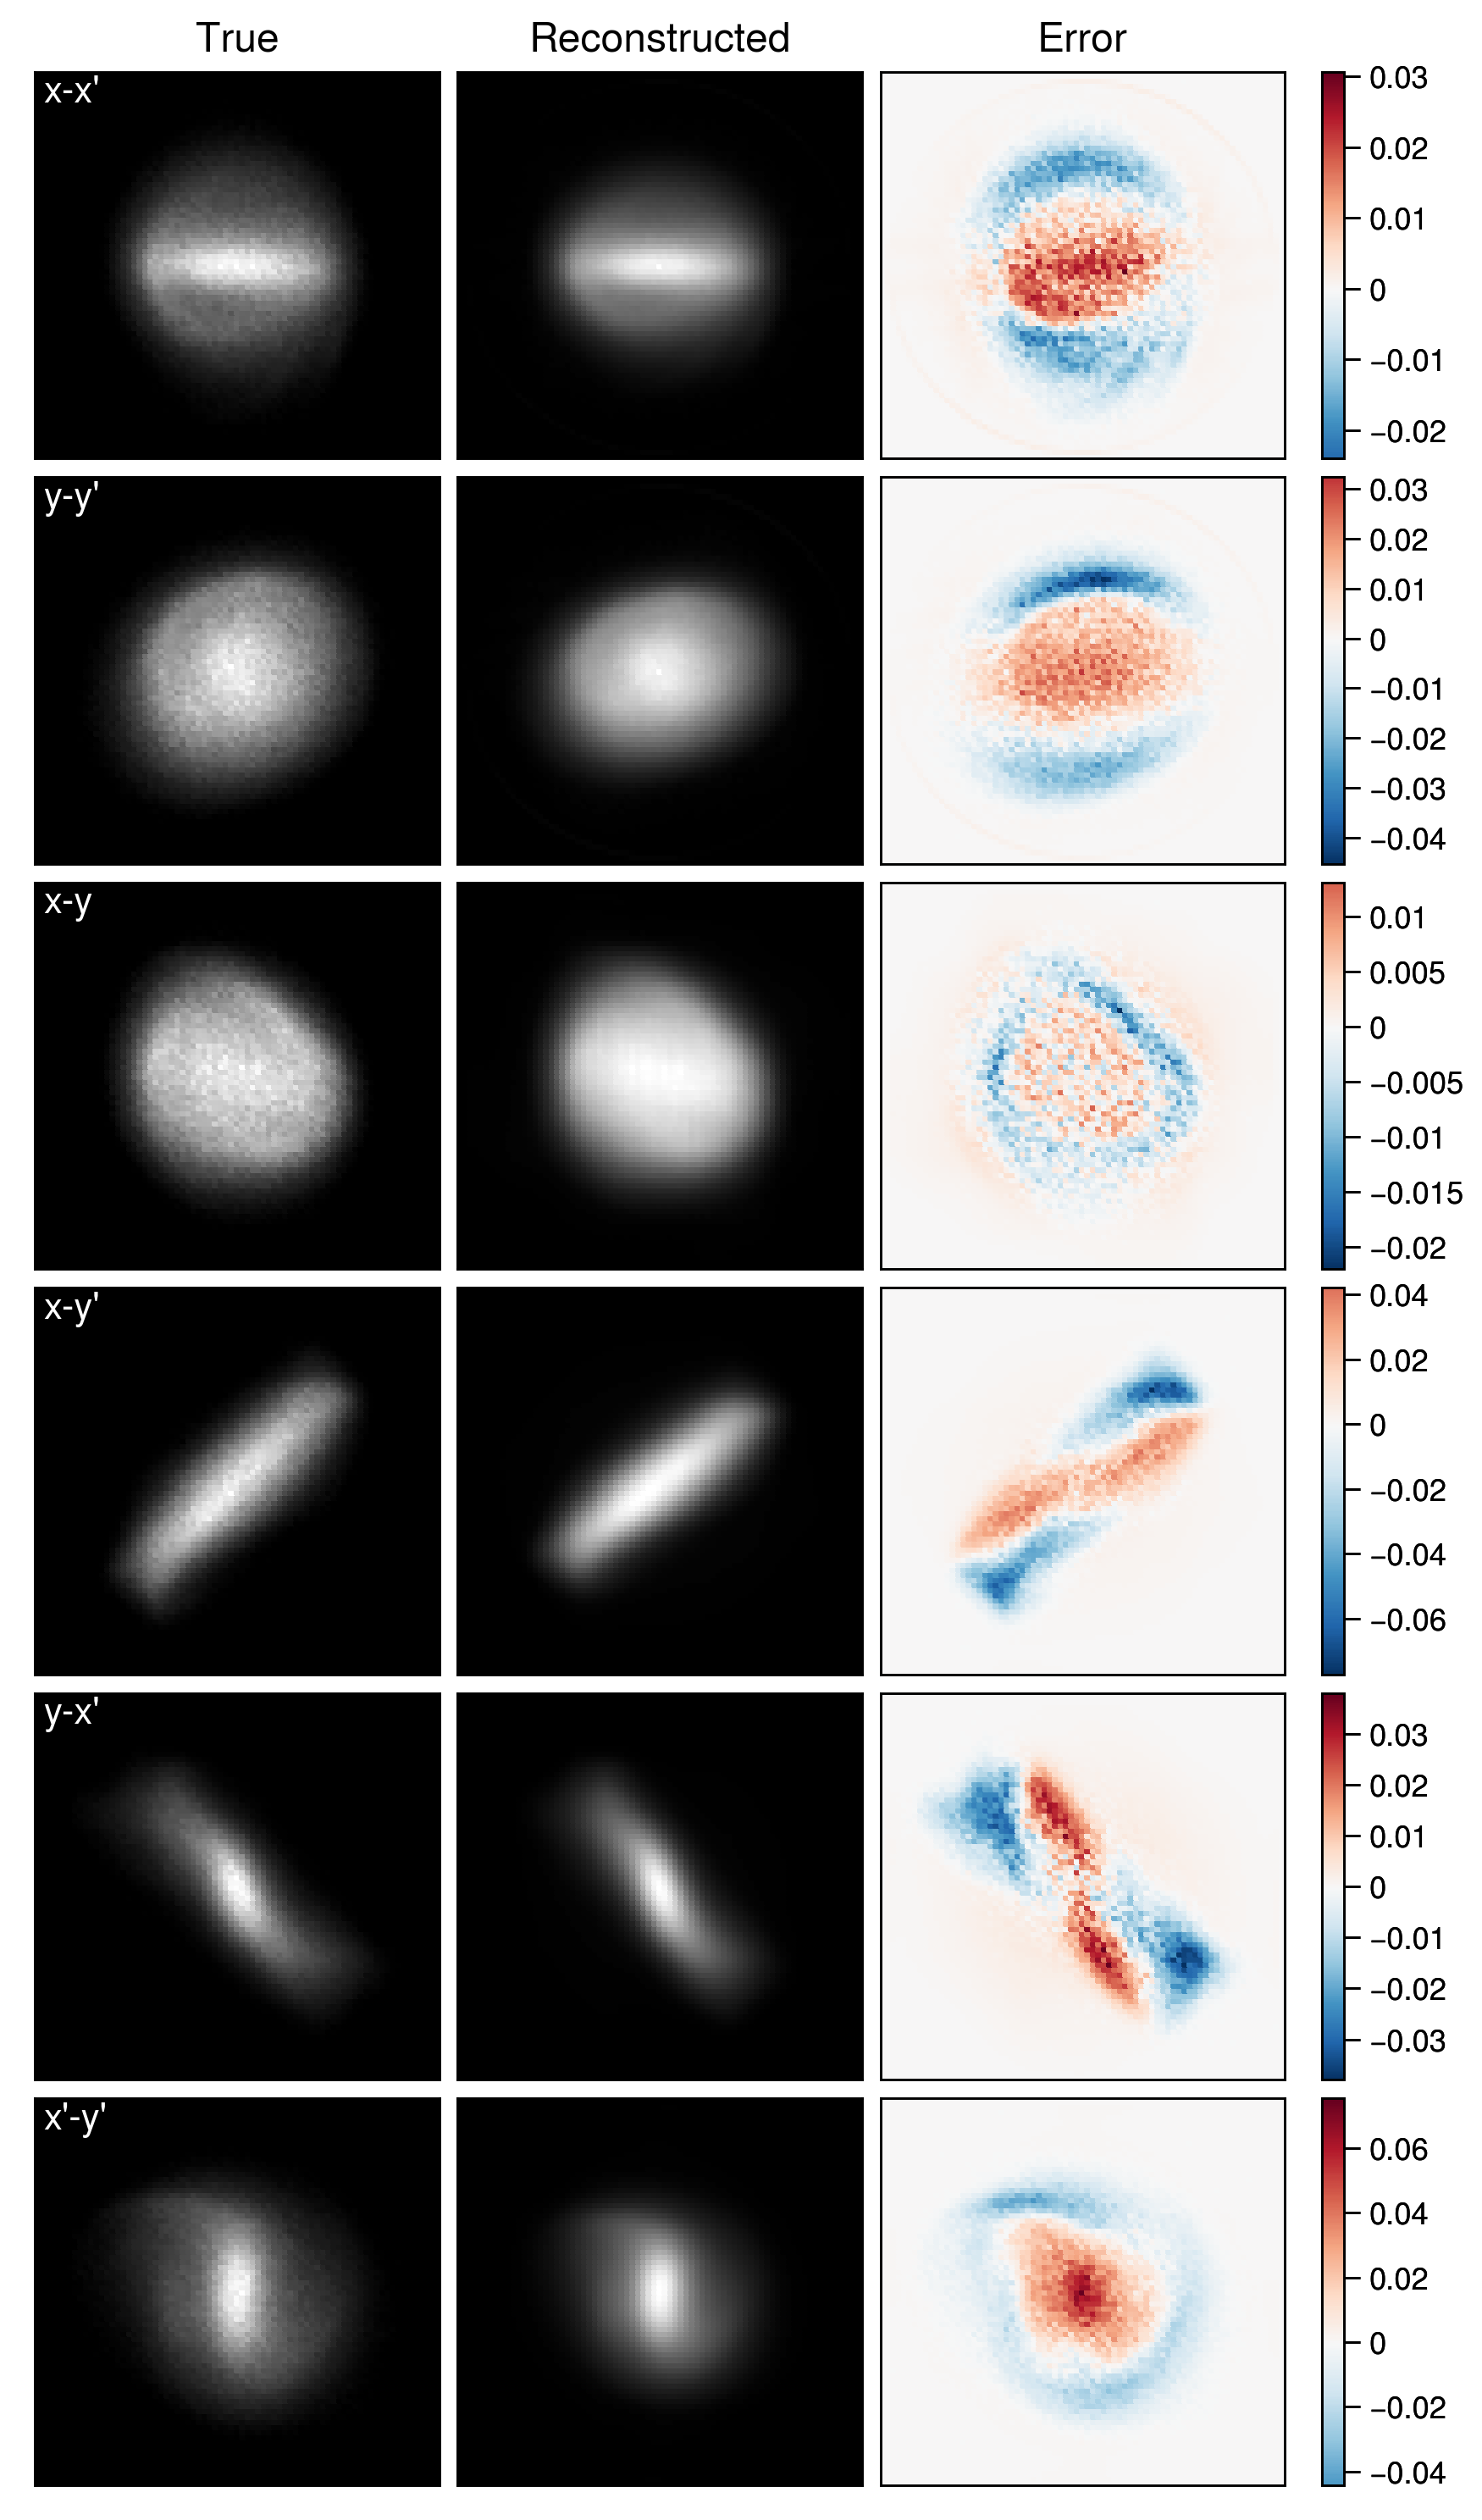
\includegraphics[width=0.8\textwidth]{Images/chapter4/tomo_sim_rec_hock_proj_2D.png}
    \caption{Simulated reconstruction using Hock's method (normalized phase space).}
    \label{fig:tomo_sim_rec_hock_proj_2D}
\end{figure}
%

This method is preferred because it leverages 2D reconstruction algorithms. Open-source implementations of these algorithms are widely available and the conditions needed for accurate reconstructions are well-understood, primarily due to the use of tomography in medical imaging. 


\subsection{Direct 4D reconstruction}

If the phase advances cannot be independently controlled or if only a very small number of projections can be collected, 2D reconstruction algorithms must be generalized to 4D. Several algorithms generalize to any number of dimensions, but they may be difficult to implement, the conditions for an accurate reconstruction may be unclear, and the time and space complexity may make the method infeasible. We focus on two methods that have recently been experimentally demonstrated.


\subsubsection{ART}

Each measured projection on the screen produces the following set of equations:
%
\begin{equation}\label{eq:art}
    \bm{\rho} = \mathbf{P} \bm{\psi}.
\end{equation}
%
$\bm{\rho}$ is a vector of the pixel intensities on the screen and $\bm{\psi}$ is a vector of the phase space coordinates on the reconstruction grid. To form $\mathbf{P}$, we place a particle at the center of each bin in the reconstruction grid and track the particles to the screen using the transfer matrix. $\mathbf{P}_{i, j} = 1$ if particle $j$ landed in bin $i$ on the screen; otherwise, $\mathbf{P}_{i, j} = 0$. The equations produced by subsequent measurements are stacked, and the resulting system of equations is solved using a sparse least squares solver. This method has been used to reconstruct the phase space distribution in the Compact Linear Accelerator for Research and Applications (CLARA), a low-energy test facility \cite{Wolski2020}.

For an $N \times N \times N \times N$ reconstruction grid, an $N \times N$ measurement grid, and $n$ measurements, $\bm{\rho}$ has $nN^2$ elements, $\bm{\psi}$ has $n N^4$ elements, and $\mathbf{P}$ has $n N^2 \times N^4$ elements. In practice, these significant storage requirements limit the resolution of the reconstruction grid to $N \approx 50$. In Fig.~\ref{fig:tomo_sim_rec_art_proj_2D}, the method was applied to the same simulated distribution, but $9 \times 9$ projections were used instead of $15 \times 15$.
%
\begin{figure}[!p]
    \centering
    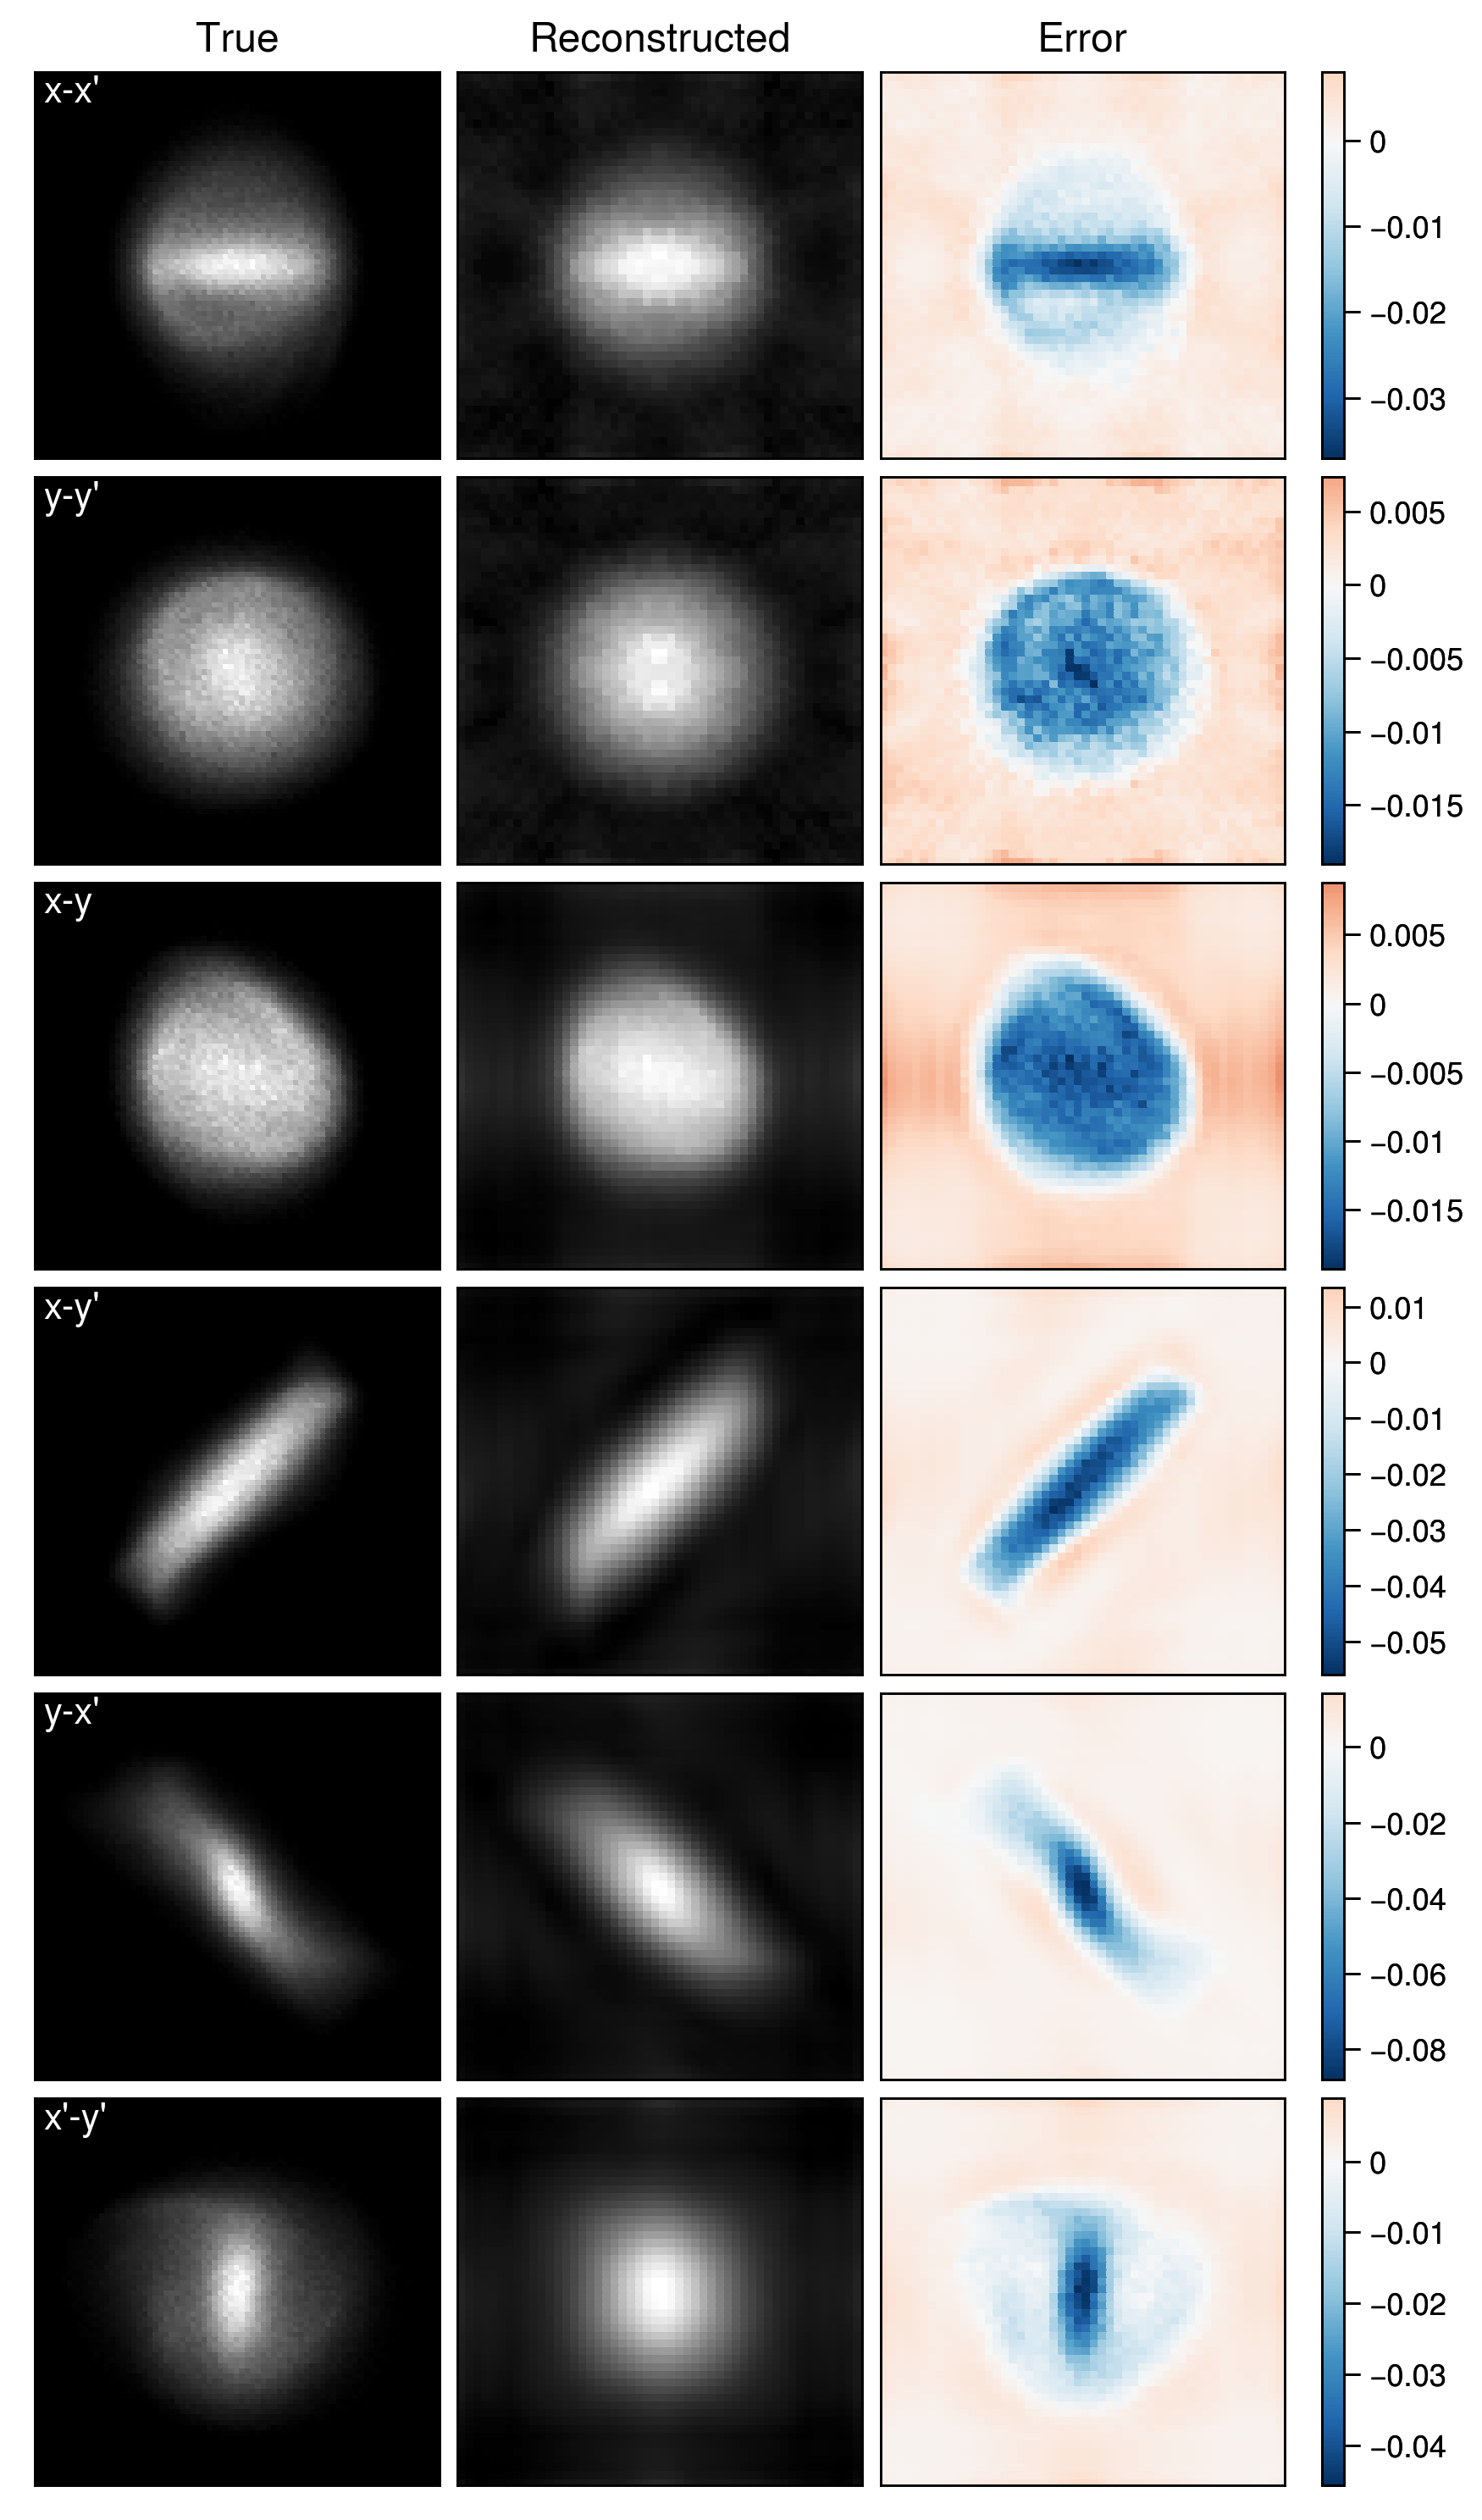
\includegraphics[width=0.8\textwidth]{Images/chapter4/tomo_sim_rec_art_proj2D.png}
    \caption{Simulated reconstruction using algebraic reconstruction (normalized phase space).}
    \label{fig:tomo_sim_rec_art_proj_2D}
\end{figure}
%
Although the main features of the distribution are present in the reconstruction, there are streaking artifacts outside the beam core that are not present in Fig.~\ref{fig:tomo_sim_rec_hock_proj_2D}, although it is likely that the performance could improve if a larger number of projections were used. Unfortunately, the algorithm took hours to execute as opposed to minutes for the previous example, even with the reduced grid resolution.


\subsubsection{Additional methods}

There are additional methods to reconstruct the 4D phase space distribution. We mention two here, although they are not used in this work.

Among the distributions consistent with the measured projections, MENT selects the distribution with the maximum entropy. For example, without any measurements constraining the solution, MENT will produce a uniform distribution. It therefore has the ability to perform well with few projections, and has been used for 2D reconstruction in particle accelerators \cite{Hock2013a}. The downside is that the iterative numerical solution is difficult to implement. In principle, the method could be extended to reconstruct the 4D phase space distribution from $x$-$y$ projections.\footnote{In principle, 4D reconstruction could be performed with 1D projections from wire-scanners \cite{Sander1979}; however, it seems a priori unlikely for this to produce an accurate result — imagine reconstructing a 3D image from 1D projections.} An analytic MENT solution has been derived and used for 4D reconstruction of an SNS minipulse from $x$-$x'$ and $y$-$y'$ projections at a laser wire \cite{Wong-forthcoming}. 

Another method is to generate a particle bunch, track the bunch to the screen, weight each particle by the measured signal at the bin where it fell on the screen, and generate new particles in the region of that particle according to its weight. The advantage of this method is that it does not assume linear transport, and that it can perform well with few projections. It was experimentally demonstrated by Wang et. al. in the Xi’an Proton Application Facility (XiPAF) using six projections \cite{Wang2019}. 



\subsection{Implementation in the SNS}

\subsubsection{Optics control}

We desire independent control of the horizontal and vertical optics. The optics control developed for the wire-scanner measurement can be used here. The constraints are now that the $\beta$ functions remain below 35 m/rad in the wire-scanner region, below 100 m/rad before the target, and stay within 15\% of their default values at the target. Fig.~\ref{fig:target_phase_scan_1} shows that the horizontal and vertical phases can both be scanned in a 180$\degree$ range, and Fig.~\ref{fig:target_phase_scan_2} overlays the $\beta$ functions and phase advances throughout the RTBT for every step in the scan. The horizontal axis starts at the first varied quadrupole and ends at the target.
%
\begin{figure}[!p]
    \centering
    \vspace*{2.0cm}
    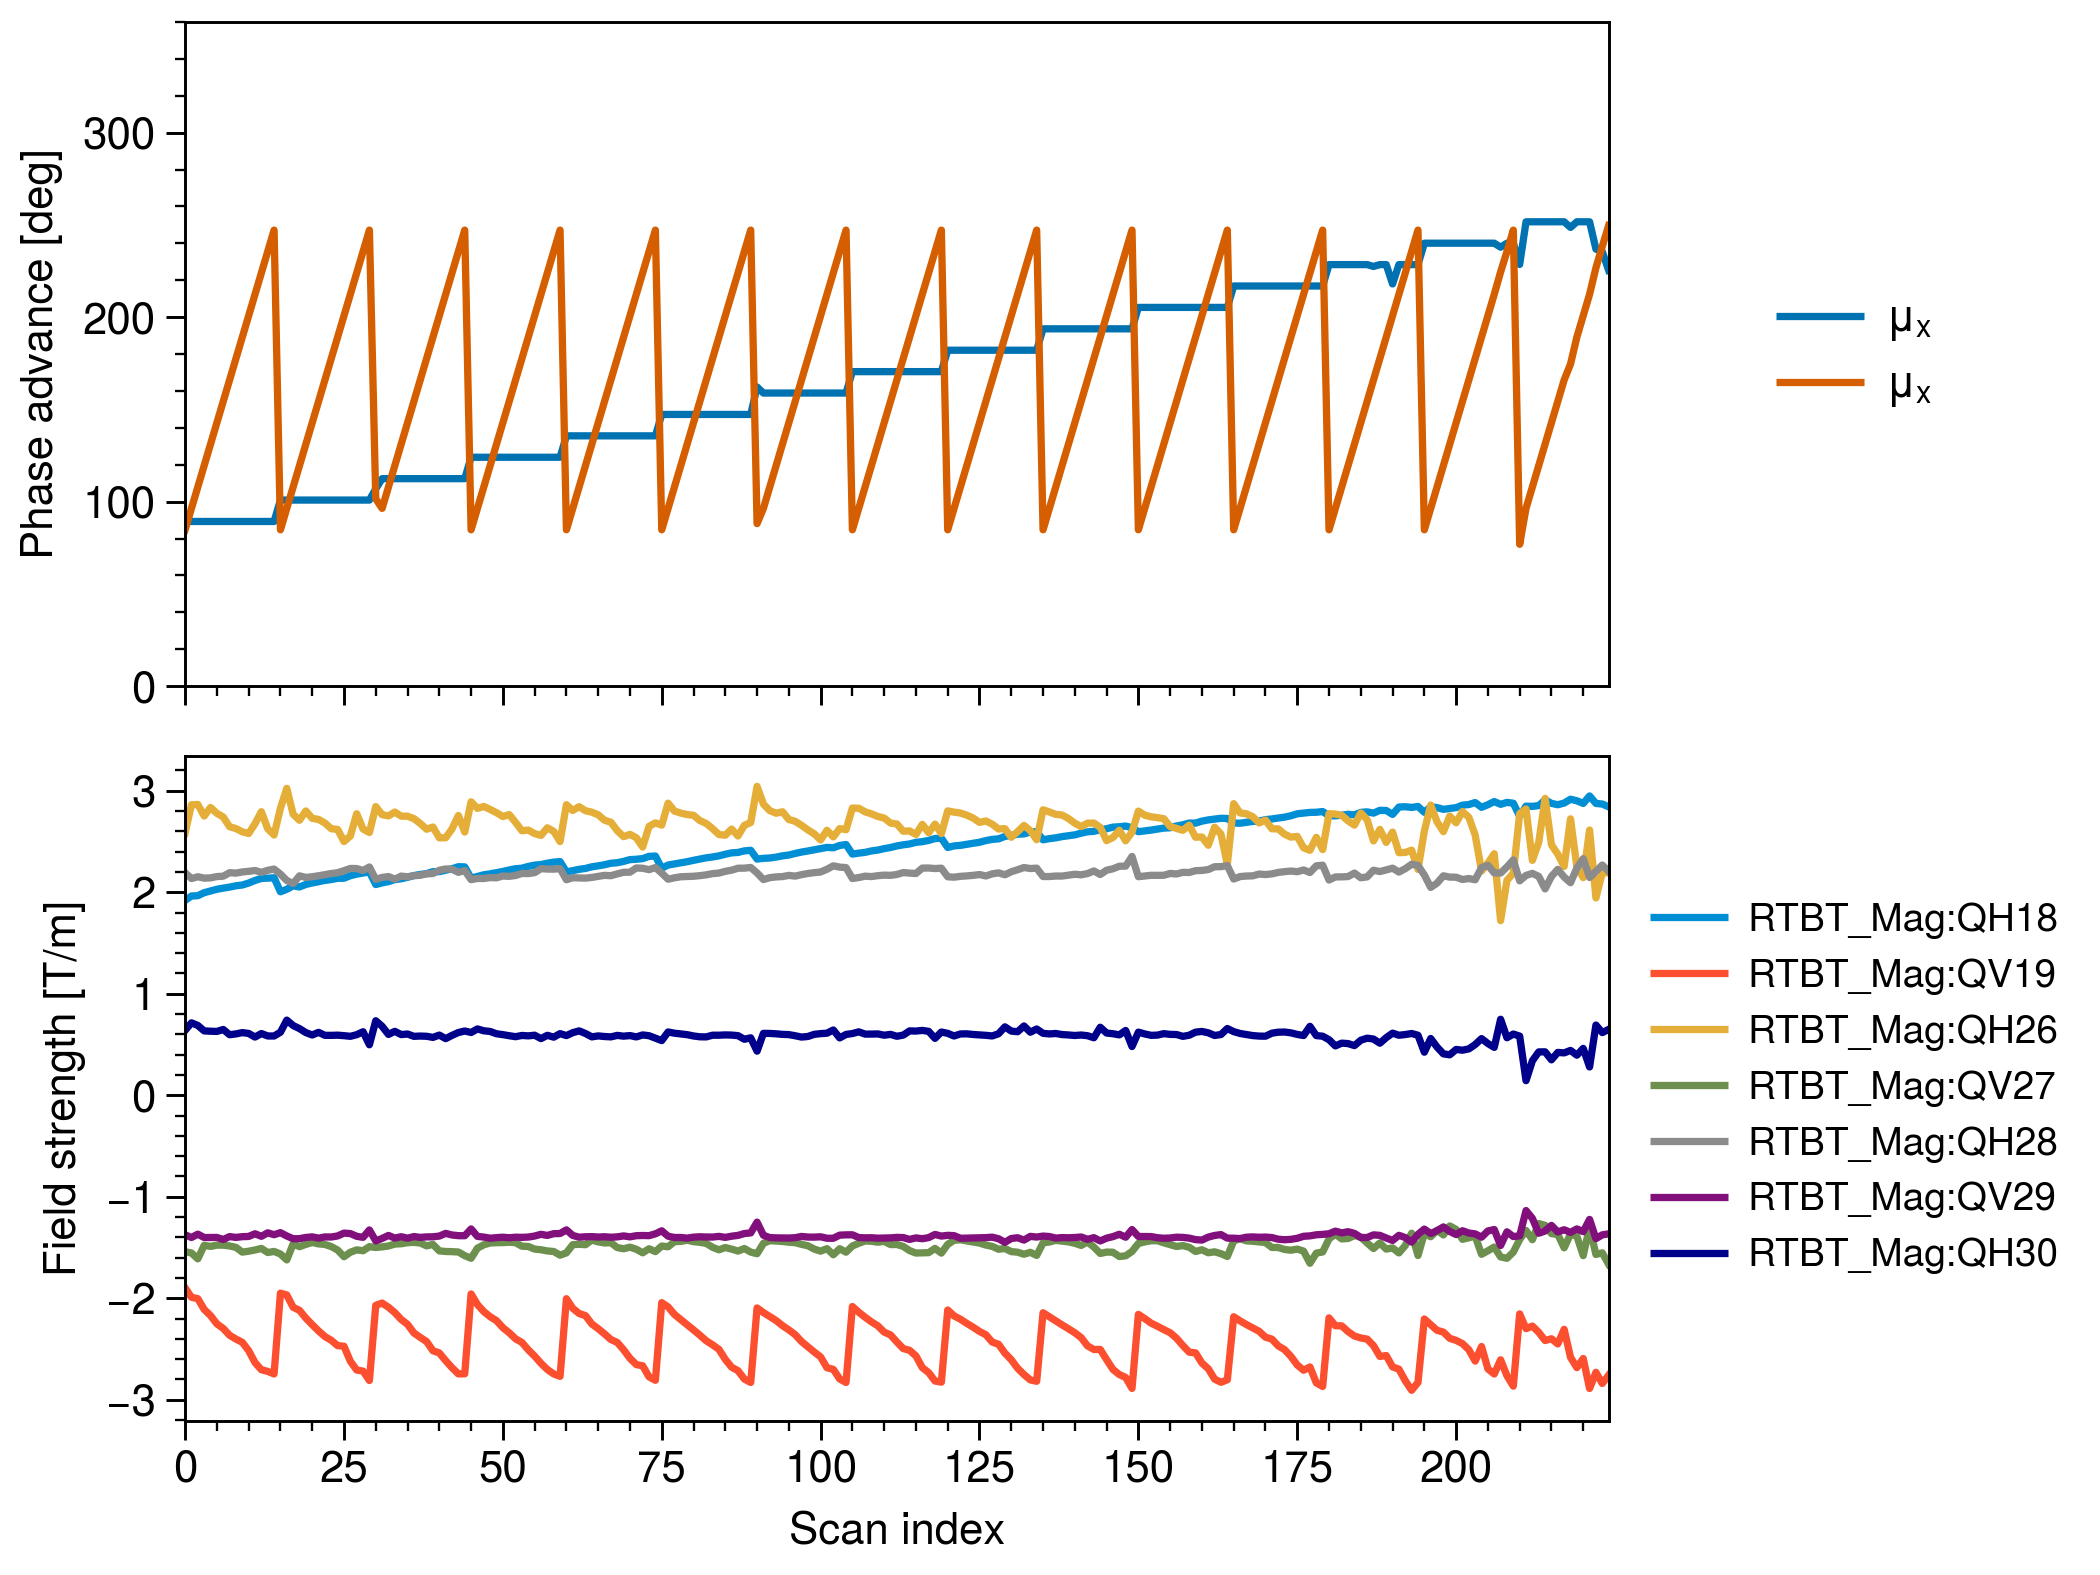
\includegraphics[width=0.9\textwidth]{Images/chapter4/target_phase_scan1.png}
    \caption{Scan of the phase advances at the target.}
     \label{fig:target_phase_scan_1}
    \vspace*{2.0cm}
\end{figure}
%
\begin{figure}[!p]
    \centering
    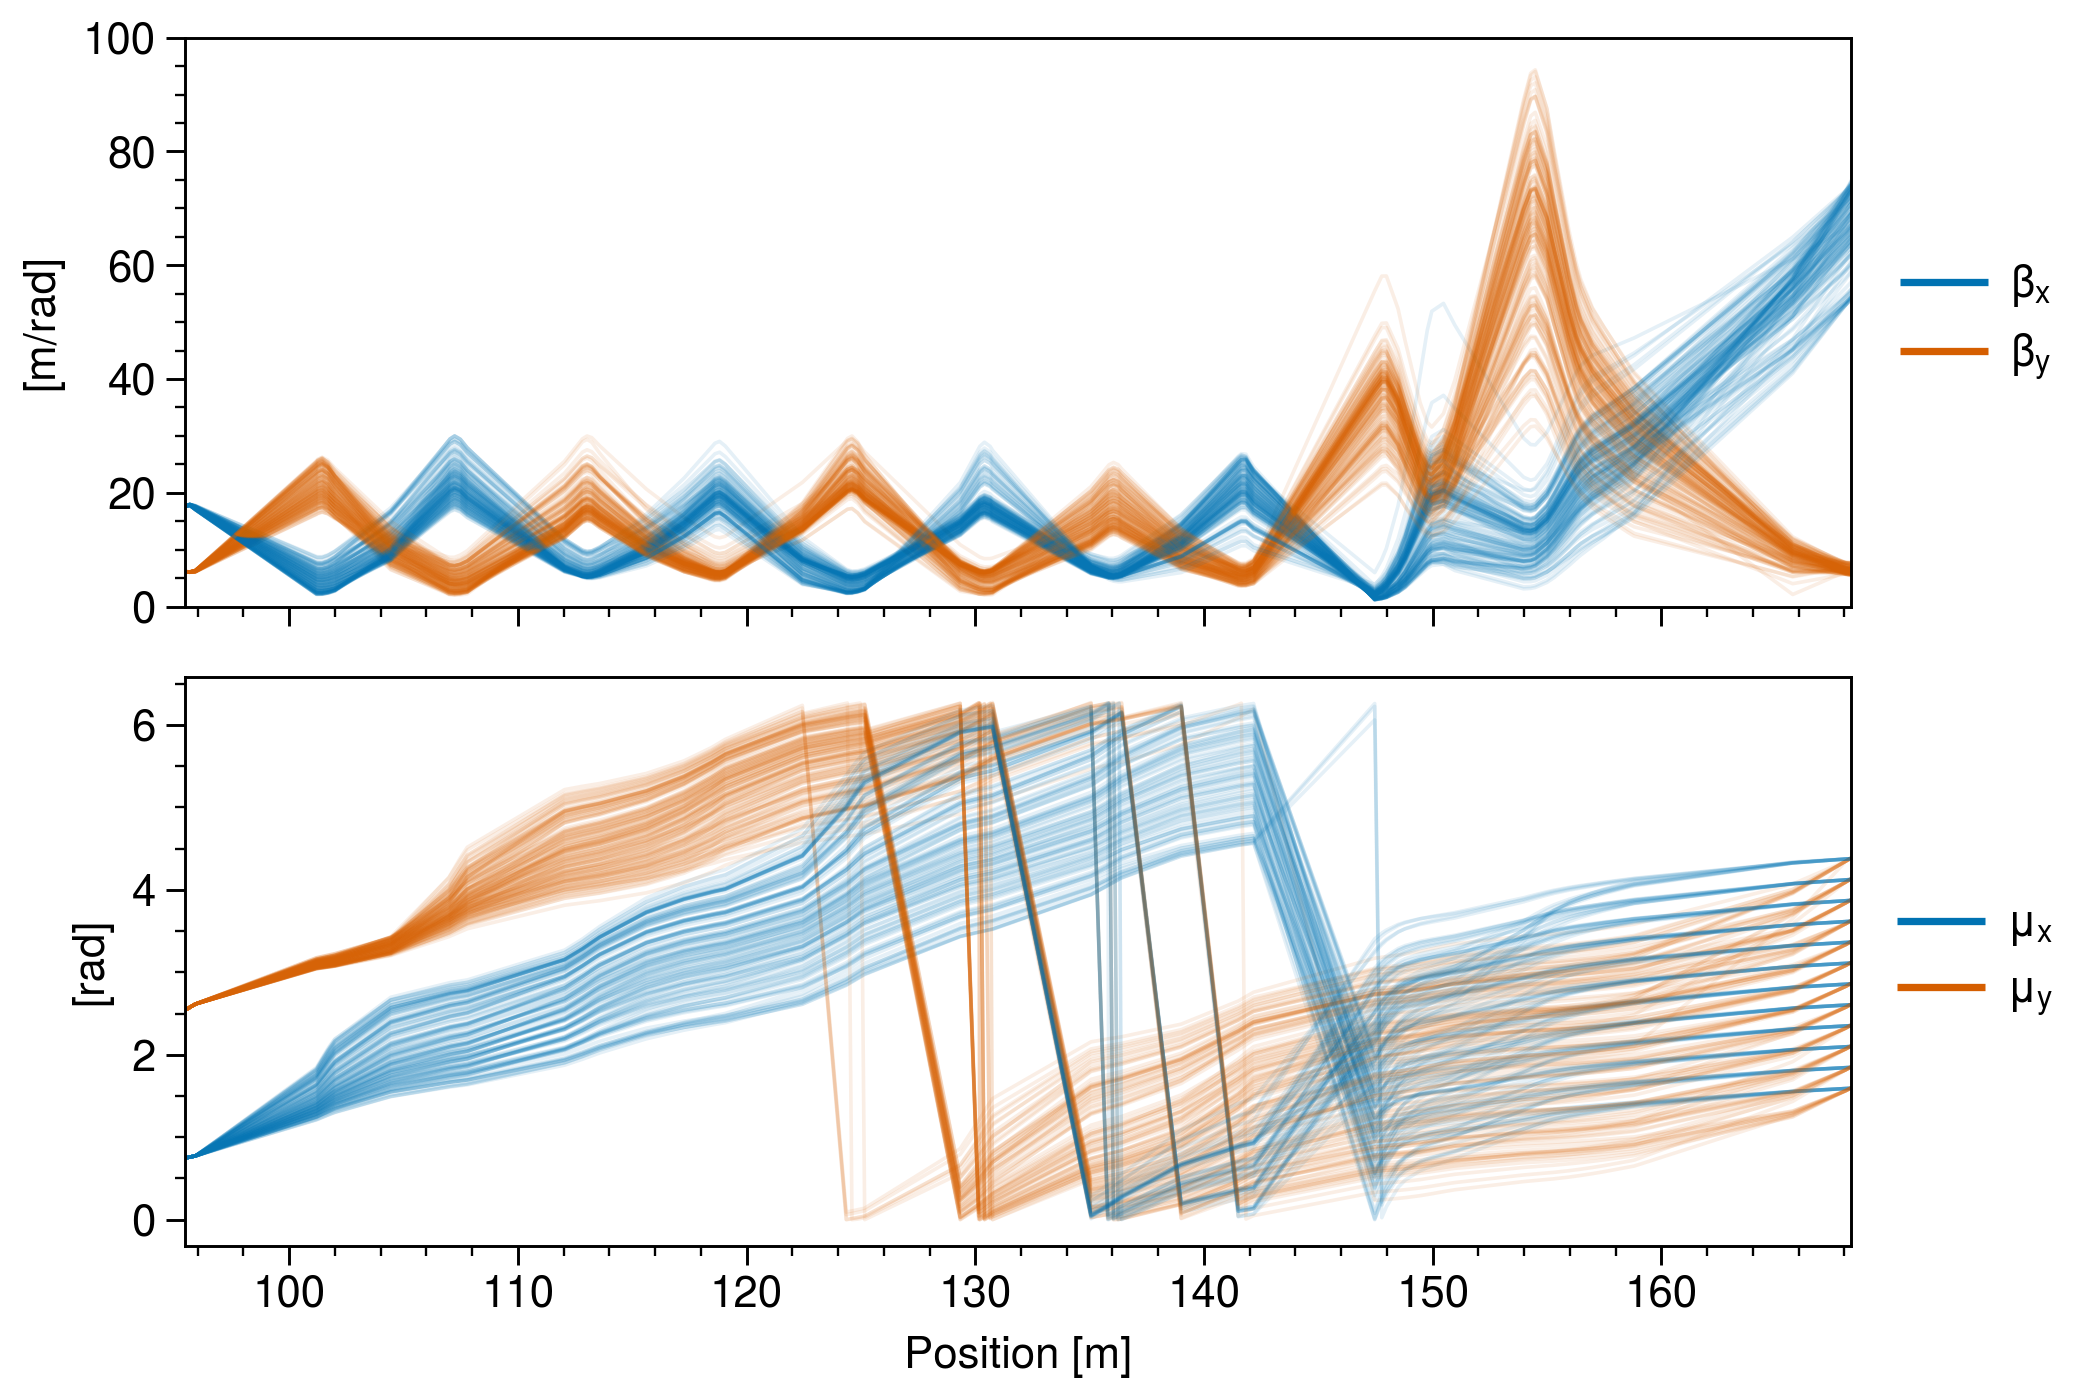
\includegraphics[width=0.9\textwidth]{Images/chapter4/target_phase_scan2.png}
    \caption{$\beta$ functions and phase advances vs. position for the scan in Fig.~\ref{fig:target_phase_scan_1}.}
    \label{fig:target_phase_scan_2}
\end{figure}
%
Computing each optics setting takes approximately sixteen seconds using an OpenXAL solver. It also takes time to change the magnet strengths in the machine, trigger the beam, and collect the target image. The time available at an accelerator physics study is 8-10 hours at a maximum, so we place an upper limit on the number of images collected during the scan at $15 \times 15$, for which it takes around one hour to calculate the optics and one hour to collect the images. 


\subsubsection{Image acquisition and processing}

Target image acquisition is handled entirely by the target imaging system software. Live target images are displayed in the SNS control room. It is straightforward to access the image from an OpenXAL script as an 80,000 element array. Thus, the script to perform the target scan repeatedly modifies the RTBT quadrupoles, triggers the beam, and saves the image array to a file.

The unprocessed target images are not ideal. First, to reduce pulse-to-pulse variation, the images can be averaged over a few pulses. Second, the beam passes through 2 meters of Helium at atmospheric pressure before the target; due to radiation damage, light from the gas appears as a streaking artifact on the lower-right of the image \cite{Blokland2010}. Although this has been corrected by delaying the shutter opening by a few microseconds, the issue has occasionally resurfaced when the beam energy is different than 1 GeV. If these images are collected, they can be identified later by placing a maximum value on the pixels far from the image center, particularly in the lower-right region. Third, there are visible grid lines from the fiber bundle. A Gaussian blur is therefore applied to the image as in Fig.~\ref{fig:target_image}. Finally, there are four dark spots on the image that serve as fiducial markers; they are visible when the beam is large. In this work, the dark spots are left in the image.
%
\begin{figure}[!p]
    \centering
    \vspace*{5cm}
    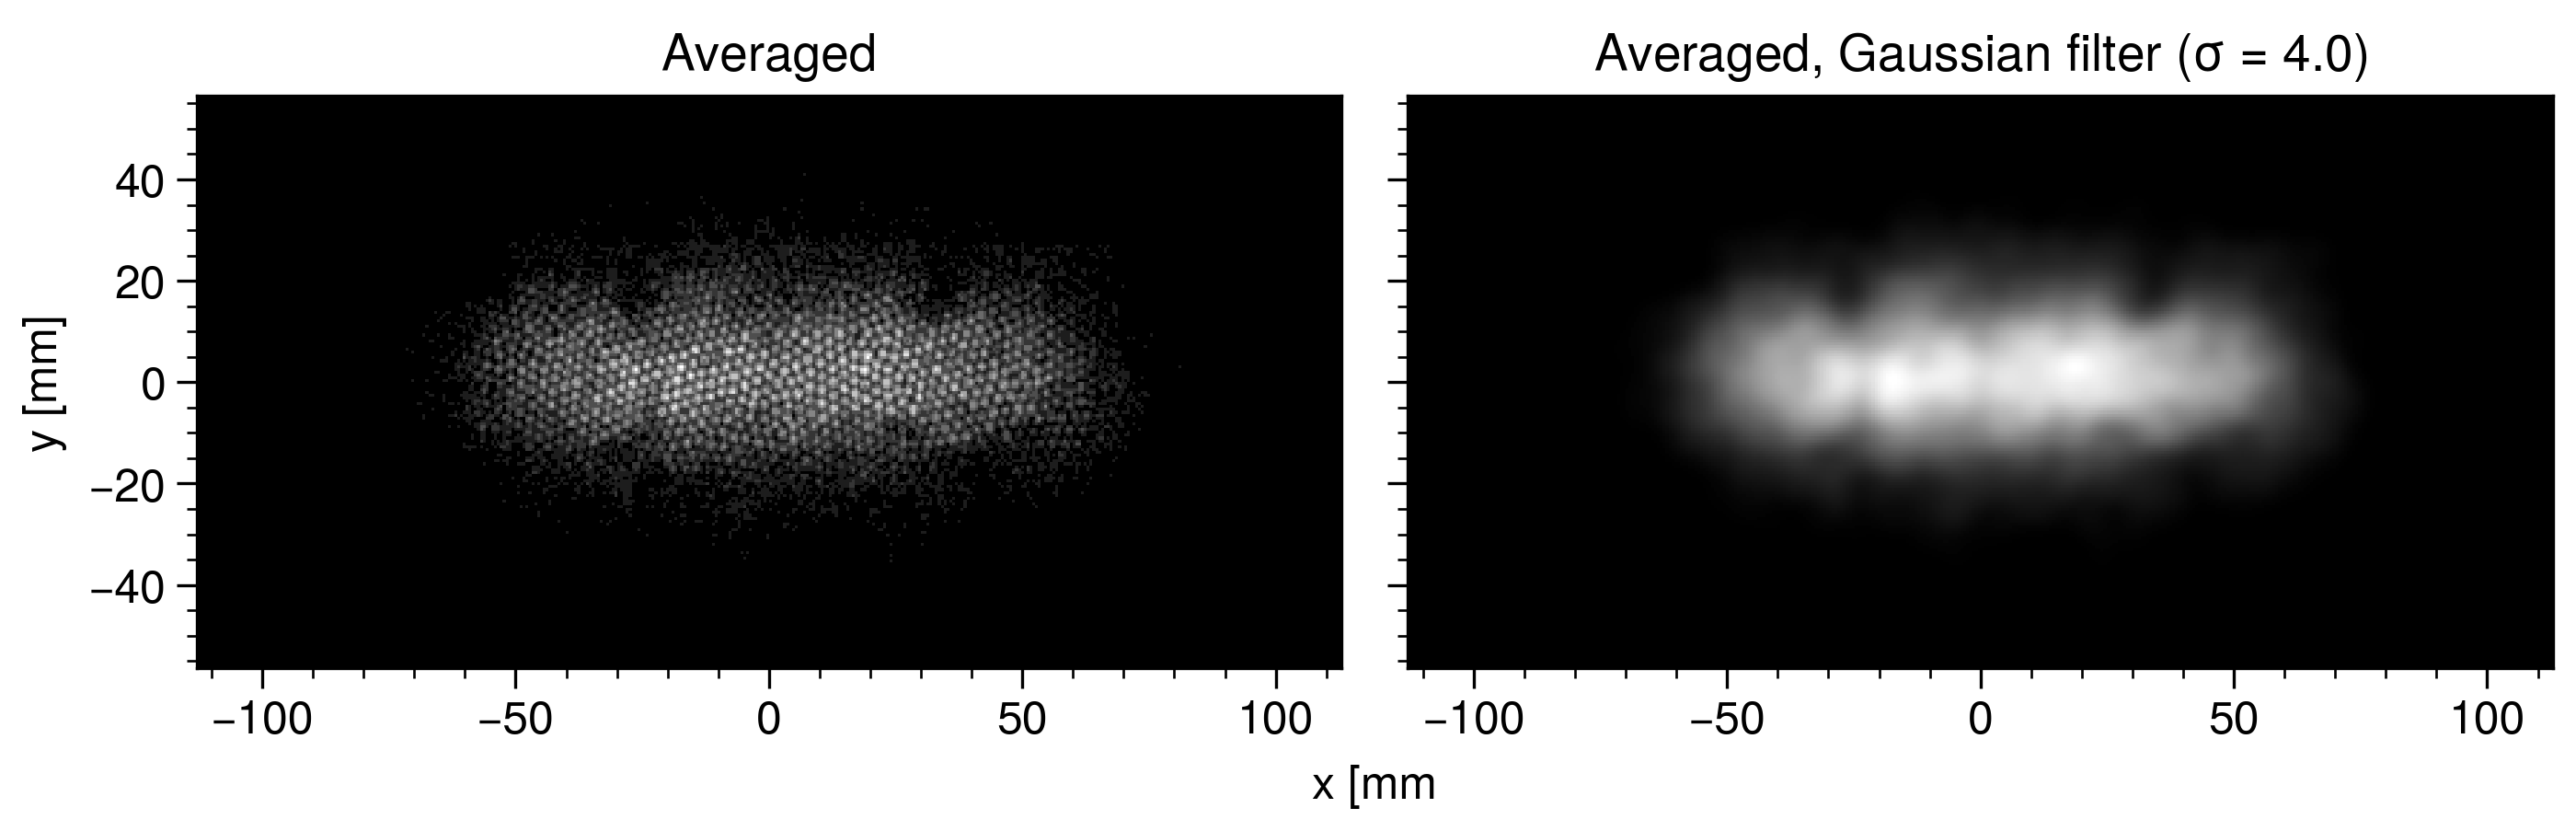
\includegraphics[width=1.0\textwidth]{Images/chapter4/target_image.png}
    \caption{Image of the beam on the target.}
    \label{fig:target_image}
     \vspace*{5cm}
\end{figure}
%


\subsubsection{Other uses of 2D projections}

There is information to be gained from 2D projections of the distribution in addition to the 4D reconstruction. The projects can be compared to an ideal uniform density ellipse. Additionally, one can observe the variation in the $x$-$y$ correlation coefficient as the difference between the horizontal and vertical phase advances is varied. This reveals any ``hidden" cross-plane correlations. In a Danilov distribution, the correlation coefficient can obtain any value in the range [-1, 1].
